\chapter{Terminology and Preliminaries}\label{ch:prelim}

\vspace*{-50pt}

\begin{figure}[ht]
        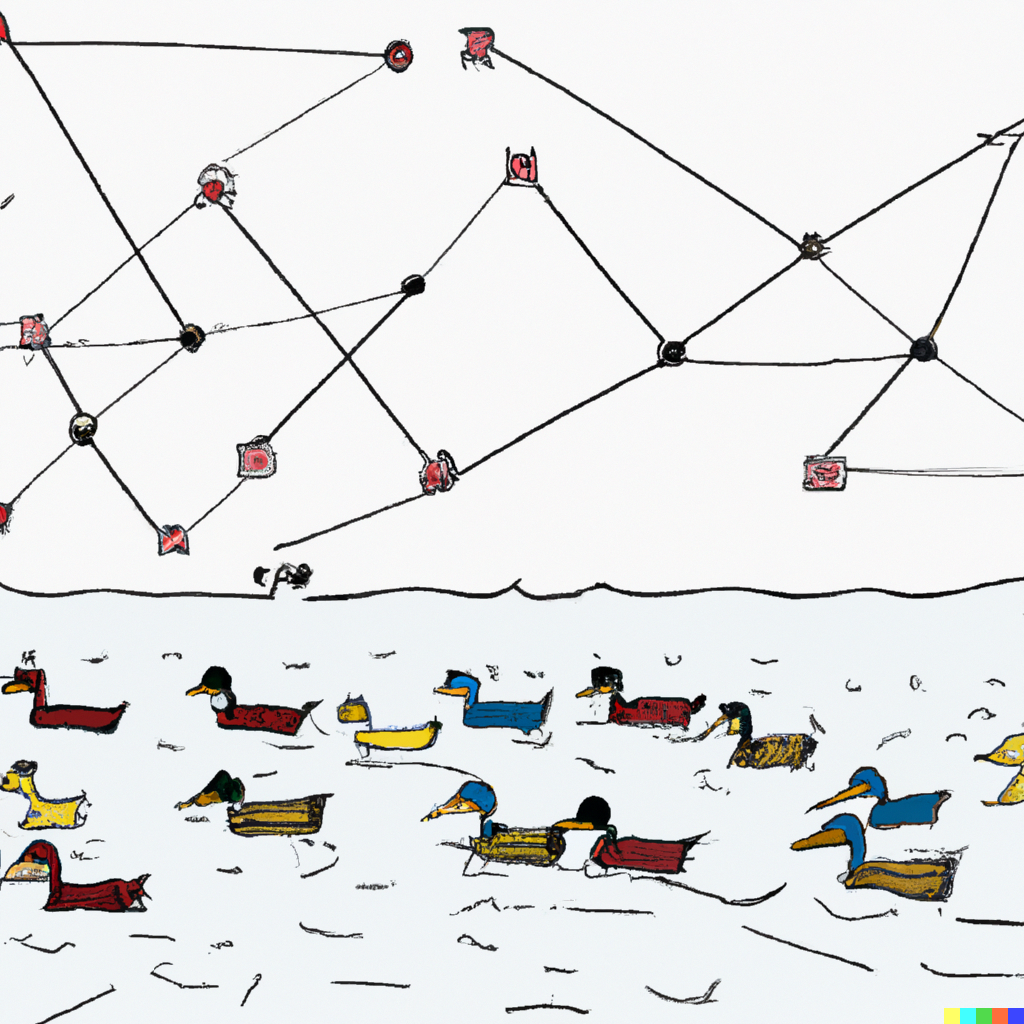
\includegraphics[width=0.35\textwidth, right]{img/gt-ducks.png}
        \captionsetup{textformat=empty,labelformat=blank}
        \caption{Generated with Dall-E. \url{https://labs.openai.com/}. ``Ducks learning graph theory while swimming on a sea sketched in color complex''}
\end{figure}

\epigraph{\itshape ``All we have to decide is what to do with the time that is given to us.''}{J. R. R. Tolkien, \textit{Gandalf} in \textit{Lord of the Rings}}


In this chapter, we will introduce the core definitions used throughout this thesis. 
Most of the definitions of graph theory are taken from \cite{Diekert2005}. 
For definitions in the area of \textit{parameterized complexity}, the book written by Cygan et al. \cite{Cygan2015} gives an excellent introduction.
For standard mathematical notation, the reader is referred to any introductory textbook into discrete mathematics (e.g. \cite{Rosen2012}).

\section{Graph Theory}

If not explicitly stated otherwise, the following definitions are taken from the book \textit{Graph Theory} written by Reinhard Diestel \cite{diestel10}.

\subsection{Basic Terminology}

\begin{definition}[Graph]
    A simple graph is a pair $G = (V, E)$ of two sets where $V$ denotes the vertices and $E \subseteq V \times V$ the edges of the graph.  A vertex $v \in V$ is incident with an edge $e \in E$ if $v \in e$. Two vertices $x, y$ are adjacent, or neighbours, if $\{x,y \} \in E$. By this definition, graph loops and multiple edges are excluded.
    
    A multigraph is a pair $(V, E)$ of disjoint sets together with a map $E \rightarrow V \cup [V]^2$ assigning to every edge either one or two vertices, its ends. Multigraphs can have loops and multiple edges.
    
    We usually denote the vertex set by $V(G)$ and its edge set by $E(G)$.


    % TODO connected 

\end{definition}

Unless stated otherwise, we usually consider only \textit{simple graphs}, but the notion of \textit{multigraphs} gets important when we later talk about the \textit{underlying multigraph} of a \dreg. 

\begin{definition}[Subgraph and Induced Subgraph]
    Let \G and $G' = (V', E')$ be two graphs. If $V' \subseteq V$ and $E' \subseteq E$ then $G'$ is a \underline{subgraph} of $G$. 
    If $G$ is a subgraph of $G'$ and $G'$ contains all the edges to $G$ with both endpoints in $V(G')$, then $G'$ is an \underline{induced subgraph} of $G$ and we write $G' = G[V(G')]$.
\end{definition}


%TODO Quote
\begin{definition}[Degrees]
    Let \G be a graph. The \textit{degree} $d_G(v)$ (shortly $d(v)$ if $G$ is clear from the context) of a vertex $v \in V$ is the number of neighbors of v. We call a vertex of degree $0$ as \underline{isolated} and one of degree $1$ as a \underline{pendant}. If all the vertices of $G$ have the same degree $k$, then $g$ is $k$-regular.
\end{definition}

% TODO Quote e.g. The open neighborhood number of a graph
\begin{definition}[Closed and Open Neighborhoods {\cite{Balakrishnan2012}}]
    Let \G be a (non-empty) graph. 
    The set of all neighbors of $v$ is the \underline{open neighborhood} of $v$ and denoted by $N(v)$; the set $N[v] = N(v) \cup \{v\}$ is the \underline{closed neighborhood} f $v$ in $G$. When G needs to be made explicit, those open and closed neighborhoods are denoted by $N_G(v)$ and $N_G[v]$. 
\end{definition}

\begin{definition}[isomorphic Graphs]
Let \G and $G' = (V', E')$ be two graphs. We call $G$ and $G'$ \underline{isomorphic}, if there exists a bijection $\phi: V \rightarrow V'$ with $\{x, y\} \in E \Leftrightarrow \phi(x)\phi(y) \in E'$ for all  $x,y \in V$. Such a map $\phi$ is called \underline{isomorphism}.

If a graph $G$ is isomorphic to another graph $h$, we denote $G \simeq H$. 
\end{definition}

\begin{definition}[Paths and Cycles]
    A path is a non-empty graph $P = (V,E)$ of the form $V = \bigcup_{i  \in [k]} \{x_i\}$ and $E = \bigcup_{i \in  [k-1]} \{x_ix_{i+1}\}$ where the $x_i$ are distinct. The vertices $x_0$ and $x_k$ are \underline{linked} by $P$ and are called the \textit{ends} of $P$. The \underline{length} of a path is its number of edges and the path on $n$ vertices is denoted by  $P_n$. We refer to a path $P$ by a natural sequence of its vertices: $P = x_0x_1...x_k$. Such a path $P$ is a path between $x_0$ and $x_k$, or a $x_0,x_k$-path.
    If $P = x_0...x_k$ is a path and $k \geq 2$, the graph with vertex set $V(P)$ and edge set $E(P) \cup \{x_kx_0\}$ is a \underline{cycle}. The cycle on $n$ vertices is denoted as $C_n$.
    The \underline{distance} $d_G(v,w)$ from a vertex $v$ to a vertex $w$ in a graph $g$ is the length of the shortest path between $v$ and $w$. If $v$ and $w$ are not linked by any path in $G$, we set $d_G(v,w) = \infty$. Again, if $G$ is clear from the context, we omit the subscripted $G$ and just write $d(v,w)$ instead.
\end{definition}

\subsection{Graph Classes}

A \textit{graph class} is a set of graphs $\mathfrak{G}$ that is closed under isomorphism that is if $G \in \mathfrak{G}$ and a $H \simeq G$ then $H \in \mathfrak{G}$ as well.

\begin{definition}[Graph Parameters]
Let \G be a graph.
An  \underline{independent set} of $G$ is a set of pairwise non-adjacent vertices. 
A \underline{clique} of $G$ is a set of pairwise adjacent vertices. 
A \underline{vertex cover} of $G$ is a subset of vertices containing at least one endpoint of every edge. 
A \underline{dominating set} is a subset $D$ of vertices such that all vertices not contained in are adjacent to some vertex in $D$.
\end{definition}

\begin{graphclass}[r-partite]
    Let $r \geq 2$ be an integer. A Graph $G = (V, E)$ is called \underline{r-partite} if $V$ admits a partition into $r$ classes such that every edge has its ends in different classes: Vertices in the same partition class must not be adjacent. 
    A \textit{$2$-partite} graph is called \underline{bipartite}. 
    
    An $r$-partite graph in which every two vertices from different partition classes are adjacent is called \underline{complete}. For the \underline{complete bipartite graph} on bipartitions $X \uplus Y$ of size $m$ and $n$, we shortly write $K_{m,n}$. 
\end{graphclass}

\begin{graphclass}[Complete]
If all vertices of a graph \G are pairwise adjacent, we say that $G$ is \underline{complete}. 
A complete graph on $n$ vertices is a $K_n$. A $K_3$ is called a \underline{triangle}.
\end{graphclass}


%\begin{definition}[{\cite[IV. Triangulated Graphs]{Berge1966}}]
%    A graph G is called \textit{chordal} (or in the older literature \textit{triangulated}) graphs if for every cycle $c = [p_1,...,p_n,p_1]$ of length $l > 3$ there is an edge of $G$ joining two non-consecutive vertices of c. Such vertices are called chords of the cycle   
%\end{definition}

\begin{graphclass}[Chordal]
For a graph \G, an edge that joins two vertices of a cycle, but is not itself an edge of the cycle is a \underline{chord} of that cycle.

Furthermore, we say $G$ is \underline{chordal} (or \textit{triangulated}) if each of its cycles of length at least four has a chord. In other words, it contains no induced cycle other than triangles.

\end{graphclass}

\begin{graphclass}[Split]
A \underline{split graph} is a graph \G whose vertices can be partitioned into a clique and an independent set.    
\end{graphclass}

%\begin{graphclass}[Bipartite {\cite[p.5]{Bondy2008}}]
%A \textit{\bg} is a Graph G whose vertex set can be partitioned into two subsets X and Y, so that each edge has one end in X and one end in Y. Such a partition (X,Y) is called a \textit{bipartition} of G.
%\end{graphclass}

%\begin{definition}[Perfect Graphs]
    
%\end{definition}

\begin{graphclass}[Planar]

A \textit{plane graph} is a pair $(V,E)$ of finite sets with the following properties:

\begin{itemize}
    \item $V \subseteq \mathbb{R}^2$ (Vertices),
    \vspace{-2mm}
    \item Every edge is an arc between two vertices, 
    \vspace{-2mm}
    \item different edges have different sets of endpoints, and
    \vspace{-2mm}
    \item The interior of an edge contains no vertex and no point of any other edge
\end{itemize}

An embedding in the plane, or \textit{planar embedding}, of an (abstract) graph $G$ is an isomorphism between $G$ and a plane graph $H$. A \textit{plane graph} can be seen as a concrete \textbf{embedding} of the planar graph into the ``plane'' $\mathbb{R}^2$.

\end{graphclass}

For an introduction into classical complexity theory. Refer to the standard textbooks aaran und cpo.
Rely an \cite[]{}
\section{Parametrized Complexity}

\paragraph{Ways to cope with NP-hard problem} Usually 

\begin{center}
    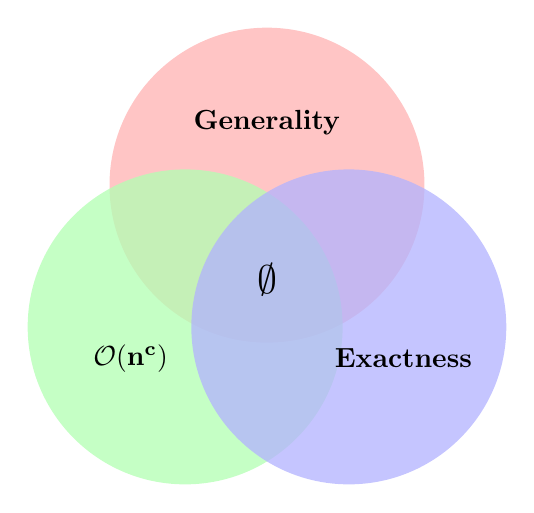
\begin{tikzpicture}
        \begin{scope}[blend mode = normal,opacity=0.75]
            \fill[red!30!white]   ( 90:1.2) circle (2);
            \fill[green!30!white] (210:1.2) circle (2);
            \fill[blue!30!white]  (330:1.2) circle (2);
        \end{scope}
        \node at ( 90:2)    {\textbf{Generality}};
        \node at ( 210:2)   {$\mathbf{\mathcal{O}(n^c)}$};
        \node at ( 330:2)   {\textbf{Exactness}};
        \node [font=\Large] {$\emptyset$};
    \end{tikzpicture}
\end{center}


\begin{definition}[Parametrized Problem{\cite[Def 1.1]{Cygan2015}}]
    A parametrized problem is a $L\subseteq\Sigma^*\times \mathbb{N}$ ($\Sigma$ finite fixed alphabet) for an instance $(x,k)\in \Sigma^*\times \mathbb{N}$, where k is called the \textit{parameter}.
\end{definition}

\begin{definition}[Instance Size]
    The \textbf{size of an instance} of an instance $(x,k)$ of a parametrized problem is $\abs{(x,k)} = \abs{x} + k$
\end{definition}
We will now clarify the basic terminology withing Parametrized Complexity. 
We are now giving a short introduction into the world of parametrized complexity. 
* General Introduction


\subsection{Fixed Parameter Tractability}

\begin{definition} [The Class FPT {\cite[Def 1.2]{Cygan2015}}]
    A parametrized problem $L\subseteq\Sigma^*\times\mathbb{N}$ is called \textit{fixed-parameter tractable} if there exists an algorithm A (called a \textit{fixed-parameter algorithm}), a computable function $f:\mathbb{N} \rightarrow \mathbb{N}$ and a constant c such that, given $(x,k) \in \Sigma^* \times \mathbb{N}$, the algorithm $\mathcal{A}$ correctly decides whether $(x,k) \in L$ in time bounded by $f(k) \cdot |(x,k)|^c$. The complexity class containing all fixed-parameter tractable problems is called \textit{FPT}
\end{definition}


\subsection{Kernelization}

\begin{definition}[kernelization Algoritm{\cite[Def 2.1]{Cygan2015}}]
A \textit{Kernelization Algorithm} or \textit{kernel} is an algorithm $\mathfrak{A}$ for a parametrized Problem Q, that given an instance $(I,k)$ of Q works in polynomial time and returns an equivalent instance $(I', k')$ of Q. Moreover, we require that $size_{\mathfrak{A}}(k) \leq g(k)$ for some computable function $g:\mathbb{N} \rightarrow \mathbb{N}$
\end{definition}

%TODO better
If we bound the size of the kernel by linear function $f(m) = \mathcal{O}(k)$, we say that the problem admits a \textbf{linear kernel}. 

%Examplary, if we reduce a graph for a graph problem in such a way that we can garuantee that our reduced graph only has a a few vertices \textbf{linear} in  $k$ left

The main idea, preprocessing algorithm, shrink size as much as possible, sound reduction rules,small output instance

\begin{definition}[Output size of a Preprocessing Procedure {\cite[p. 18]{Cygan2015}}] The output size of a preprocessing algorithms $\mathfrak{A}$ is defined as 

    \[\mathrm{size}_{\mathfrak{A}}(k) = \sup\{\abs{I'} + l': (I',k')= \mathfrak{A}(I,k), I \in \Sigma^* \} \]
\end{definition}

possibly infinite

Clearly, if there exists a kernelization algorithm for a problem $L$ and an algorithm $\mathfrak{A}$ with any runtime to decide $L$, the problem is in $FPT$ because after the kernelization pre-processing has been applied, the size of the reduced instance is a function merely in $k$ and independent of the input size $n$. In \cref{ch:linkern} we will explicitly construct a kernel for \psdom and hence showing it to be in \textit{FPT}. 

% Interstingly, als the converse?

\begin{definition}[Reduction Rules {\cite[p. 18]{Cygan2015}}]
A \textbf{reduction rule} is a function $\phi:\Sigma^* \times \mathbb{N} \rightarrow \Sigma^* \times \mathbb{N}$ that maps an instance $(x,k)$ to an equivalent instance $(x',k')$ such that $phi$ is computable in time polynomial in $\abs{x}$ and $k$
\end{definition}

\begin{definition}[Equivalent Instance {\cite[p. 18]{Cygan2015}}]
     This is a test
\end{definition}

\begin{definition}{Soundness of a rule}

\end{definition}

A \textbf{reduction rule} is a function $\Sigma* \times \mathbb{N}$ that maps an instance $(x,k)$ to an equivalent instance $(x',k')$ such that xx is computable in time polynomial in $\abs{x}$ and $k$

\subsection{Fixed Parameter Intractability: The w-Hierarchy}
\subsection{Compare to classical NP-Hardness theory}

\subsubsection{Parametrized Reductions}
\begin{definition}[Parametrized Reduction {\cite[Def 13.1]{Cygan2015}}] Let $A,B\subseteq \Sigma^*\times\mathbb{N}$ two parametrized problems. A \textit{Parametrized Reduction} from A to B is an algorithm that, given an instance $(x,k)$ of A, outputs an instance $(x', k')$ of B such that

    \begin{itemize}
        \item $(x,k)$ is a \textcolor{gray}{yes instance} of A \textbf{iff} $(x',k')$ is a \textcolor{gray}{yes instance} of B
        \item $k' \leq g(k)$ for some computable function $g$
        \item the running time is $f(k)\cdot |x|^{\mathcal{O}(1)}$ (FPT!)
    \end{itemize}
\end{definition}
    \subsubsection{The $w$-hierarchy}



\chapter{On Parameterized Semitotal Domination}\label{ch:semitotal-domination}

\vspace*{-50pt}

\begin{figure}[ht]
        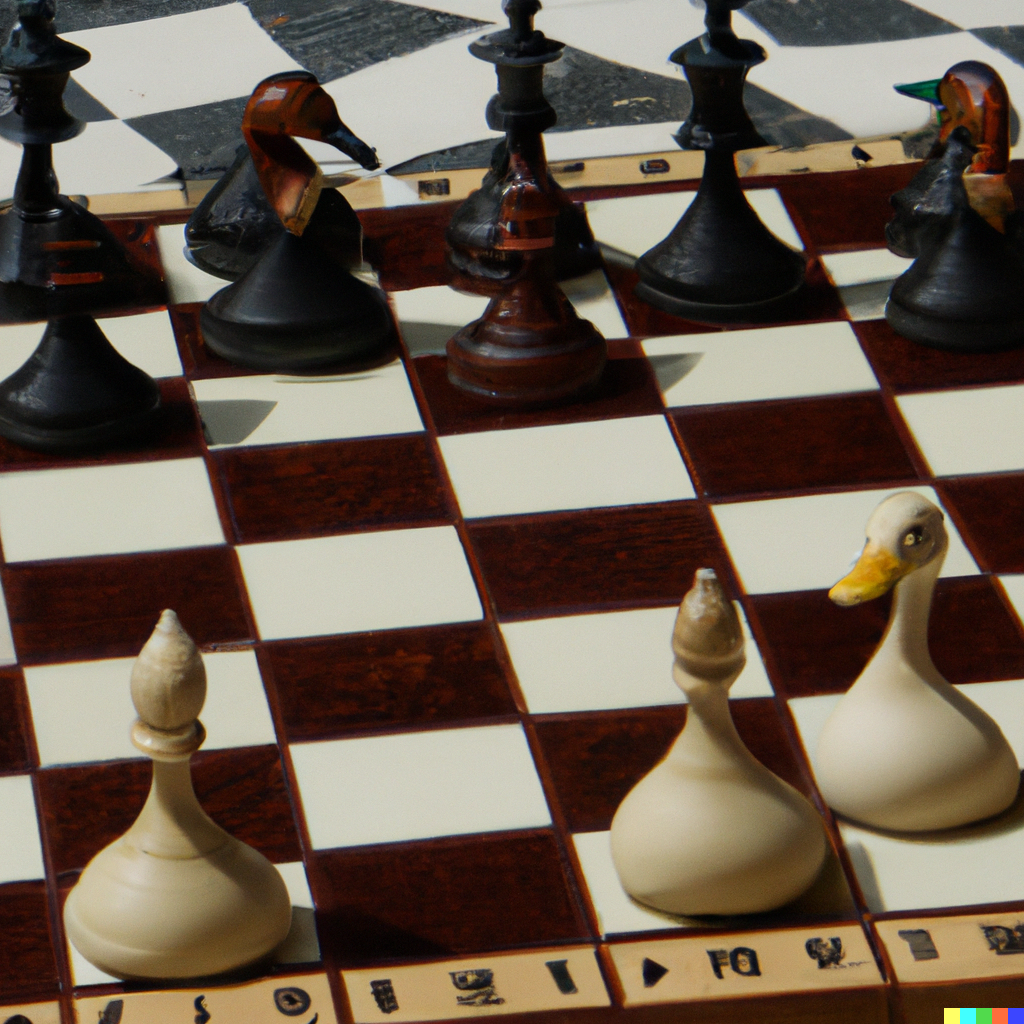
\includegraphics[width=0.35\textwidth, right]{img/chess.png}
        \captionsetup{textformat=empty,labelformat=blank}
        \caption{Generated with Dall-E. \url{https://labs.openai.com/}. ``Duck playing chess''}
\end{figure}

%\epigraph{\itshape In computer science, parameterized complexity is a framework for studying the complexity of computational problems, in which the complexity of a problem is not just a function of the size of the input, but also a function of one or more additional parameters that describe the problem instance. }{chatGPT, \textit{2022}}
% Maybe add some sentences from here: https://link.springer.com/content/pdf/10.1007/978-1-4419-7997-1.pdf?pdf=button p.243
\epigraph{\itshape TODO: Make a nice chatGPT poem.}{chatGPT, \textit{2022}}

In connection with various chessboard problems, the concept of domination can be traced back to the mid-1800s.
For example, De Jaenosch attempted in 1862 to solve the minimum number of queens required to fully cover an $n \times n$-chessboard \cite{Jaenisch1862}.
Because of the immense amount of publications related to domination that followed, Haynes, Hedetniemi, and Slater started a comprehensive survey of the literature in 1998 \cite{Haynes1998, Haynes1998b}. 
20 years later, by a series of three more books, Haynes, Henning and Hedetniemi complemented the survey with the latest developments \cite{Haynes2020, Haynes2021, Haynes2022}.

We are now introducing the problems of \dom, \sdom and \tdom and dedicate the rest of the chapter to giving a current status about the complexity status of various graph classes. 

% We will see that most cases mirror each other for the three different problems, but sometimes there seems to be 

% Surprisingly, there are cases where the complexity of \dom and \tdom differes (e)
%If both \dom and \tdom are already hard for a class, we already have a strong assumption that this also holds for \sdom as well.

%Interestingly, most of them mimic each other for one specific class, but there are some exceptions, where this is not the case.

\section{Domination Problems}

We are now going to define the three most important domination problems for this work: \dom, \sdom and \tdom.
Recall that a dominating set of a graph \G is a subset $D \subseteq V$, such that every vertex $V \setminus D$ is adjacent to some vertex in $D$.
We say that a vertex $d$ is a \textit{dominating vertex} or \textit{dominator} if $d \in D$ and that $d$ \textit{dominates} all of its neighbors.

The \dom problem asks for a subset $D$ of size at most $k$ of vertices whose set of neighbors are adjacent o all the other vertices.
In other words: every vertex $v \notin D$ needs to have at least one neighbor in $D$.

\begin{prb}[\DOM~{\cite[p. 586]{Cygan2015}}]{prb:ds}
    \begin{tabularx}{1.0\textwidth}{>{\hsize=0.30\hsize}X>{\hsize=0.8\hsize}X}
        \textbf{Input} & Graph \G, $k \in \mathbb{N}$\\
        \textbf{Question} & Is there a set {$X \subseteq V$} of size at most $k$ such that ${N[X] = V}$? \\
    \end{tabularx}
\end{prb}

If we also demand the dominating vertices to be dominated, need the notion of \tdomin.
The \tdom problem adds one additional constraint: Every vertex $v \in D$ in the dominating set must also be dominated by some vertex $v' \in D$ which we call the \textit{witness} of $v$.

\begin{prb}[\TDOM~{\cite[p. 596]{Cygan2015}}]{prb:sds}
    \begin{tabularx}{1.0\textwidth}{>{\hsize=0.30\hsize}X>{\hsize=0.8\hsize}X}
        \textbf{Input} & Graph \G, $k \in \mathbb{N}$\\
        \textbf{Question} & Does there exists a set $X \subseteq V$ with $\abs{X}\leq k$ vertices such that for every $u \in V(G)$ there exists $v \in X$ with $\{u,v\} \in E$? \\
    \end{tabularx}
\end{prb}

Finally, \sdomin was introduced by Goddard, Henning and McPillan \cite{Goddard2014} as a relaxation of \tdomin. 
Assume that we have an arbitrary dominating set $D$ for some (connected) graph \G that has size at most two.
It is easy to observe that for each $v \in D$ there must be at least one other dominating vertex $v' \in D$ that is at most three steps away because otherwise, this would not be a dominating set. 
On the other side, by definition of a total dominating set $D$, every dominating vertex $d \in D$ has another vertex in $d' \in N(d) \cap D$ that is also dominating.
It is natural to ask what happens if we restrict this distance property to be at most two, which leads us straight to the idea of \sdomin.
For a semitotal dominating set $D$, we say that $v$ witnesses $v'$ if $v,v' \in D$ and $d(v,v') \leq 2$.

\begin{prb}[\SDOM~{\cite{Goddard2014}}]{prb:tds}
    \begin{tabularx}{1.0\textwidth}{>{\hsize=0.30\hsize}X>{\hsize=0.8\hsize}X}
        \textbf{Input} & Graph \G, $k \in \mathbb{N}$\\
        \textbf{Question} & Is there a subset $X \subseteq V$ with $\abs{X} \leq k$ such that ${N[X] = V}$ and for all $d_1 \in X$ there exists another $d_2 \in X$ such that ${d(d_1, d_2) \leq 2}$?\\
    \end{tabularx}
\end{prb}

\Cref{fig:dsexamples} demonstrates that the minimum ds, sds and tds can strictly differ in the size on a fixed graph \G. a minimum ds (left) does not need any witnesses at all and we can choose $d_1$ and $d_2$ to dominate the graph. 
As $d(d_1, d_2) = 3$, we have to introduce additional dominating vertices for a minimum sds (middle) and tds (right). 
Their only purpose is, to bridge the gap between $d_1$ and $d_2$.
% In a sds it is enough to use $d_3$, because $d(d_2,d_3) < d(d_1, d_3) \leq 2$.

\begin{figure}
     \begin{equation*}
         \tikzfig{fig/tikz/ds-examples}
     \end{equation*}
    \caption[An example for various dominating sets]{\textit{An example for a minimum dominating set, semitotal dominating set and a total dominating set, where $\gamma(G) < \gamma_{2t}(G) < \gamma_t(G)$ are strict. In the first case, only two vertices suffice to dominate all others. In the second one, we need a witness between $d_1$ and $d_2$ that is at most distance two. In the last case, $d_1$ and $d_2$ both need a neighbor in the total dominating set.}}
    \label{fig:dsexamples}
\end{figure}


\begin{definition}[Domination Numbers]
   The \underline{domination number} in a graph $G$ is the minimum cardinality of a dominating set (ds) of $G$, denoted as $\gamma(G)$. 
   The \underline{total domination number} is the minimum cardinality of a total dominating set (tds) of $G$, denoted by $\gamma_t(G)$.
   The \underline{semitotal domination number} is the minimum cardinality of a semitotal dominating set (sds) of $G$, denoted by $\gamma_t(G)$.

   We say that a ds $D$ is \underline{minimal} if no proper subset $S' \subset S$ is a ds and that $D$ is a \underline{minimum} if it is the smallest ds.
\end{definition}

Because any tds is also an sds and every sds is also a ds, $\gamma{t2}$ is squeezed between $\gamma$ and $\gamma_t$.
The  following fact was first observed by Goddard and Henning \cite{Goddard2014}:

\begin{fact}
For every graph $G$ with no isolated vertex, $\gamma(G) \leq \gamma_{t2}(G) \leq \gamma_t(G)$
\end{fact}
It turns out that for some graphs, all of these inequalities are strict. See \cref{figd:dsexamples} for an example, where $\gamma < \gamma_{t2} < \gamma_t$ and therefore.

\section{Complexity Status of \sdom}\label{ch:complexity-status}

This chapter complements the complexity status of \sdom surveyed by Galby et. al \cite{Galby2020} with the latest developments and adds the corresponding parameterized complexities. 
It is interesting to see, how most of the results are mirrored across \dom, \sdom and \tdom.
If not mentioned otherwise, our problem is always parameterized by solution size.

In the meanwhile, new polynomial time algorithms have been shown for \textit{dually chordal}, \textit{strongly chordal} \cite{Tripathi2021}, \textit{AT-free} \cite{Kloks2021} and \textit{block} \cite{Henning2022} graphs.
Furthermore, a linear time algorithm has been found for interval graphs \cite{Pradhan2021} beating the previous $\mathcal{O}(n^2)$ algorithm given by Henning and Pandey \cite{Henning2019}.

On the negative side, \sdom on \textit{circle graphs} graphs and \textit{undirected path graphs} is \NPc. 

% TODO: Make table out of that
All complexigty results are shown in \cref{tab:complexities}.

% Some words to parameterized complexity

\begin{center}
    % Add girth results: https://link.springer.com/content/pdf/10.1007/978-1-4614-6525-6.pdf?pdf=button

\resizebox{1.0\textwidth}{!}{
    \begin{tabularx}{1.8\textwidth}{lllllll}

        \arrayrulecolor{TUMBlue}\toprule
        \textbf{Graph Class}                  & \multicolumn{2}{c}{\textbf{\dom}}                       & \multicolumn{2}{c}{\textbf{\sdom}}           & \multicolumn{2}{c}{\textbf{\tdom}}                                                                                                                                \\
        \cmidrule(lr){2-3} \cmidrule(lr){4-5} \cmidrule(lr){6-7}
                                              & classical                                               & Parameterized                                & classical                                               & Parameterized              & classical                                    & Parameterized               \\
        bipartite                             & \NPcs \cite{Bertossi1984}                               & \WTWOhs                                      & \NPcs \cite{Henning2019}                                & \WTWO (this)             & \NPcs \cite{Pfaff1983}                       &                             \\
        
        line graph of bipartite               & \NPcs \cite{Korobitsin1992}                             & TODO                                         & \NPcs \cite{Galby2020}                                  &                            & \NPcs \cite{McRae1995}                       &                             \\
        
        circle                                & \NPcs \cite{Keil1993}                                   & \WONEhs \cite{Bousquet2012}                  & \NPcs \cite{Kloks2021}                                  & \textbf{Open} & \NPcs \cite{McRae1995}                       & \WONEhs \cite{Bousquet2012} \\
        
        chordal                               & \NPcs \cite{Booth1982}                                  & \WTWOhs \cite{Raman2008}                     & \NPcs \cite{Henning2019}                                & \WTWO (this)               & \NPcs \cite{Laskar1983}                      &                             \\
        
        $s$-chordal                           & \NPcs \cite{Liu2011}                                    & \WTWOhs \cite{Liu2011}                       & XXX                                                     & XX                         & \NPcs \cite{Liu2011}                         & \WONEhs \cite{Liu2011}      \\
        
        split                                 & \NPcs \cite{Bertossi1984}                               & \WTWOhs XXXX false! \cite{Raman2008}         & \NPcs \cite{Henning2019}                                & \WTWOhs Lemma XX             & \NPcs \cite{Laskar1983}                      & \WONEhs \cite{Chang1998}    \\
        
        3-claw-free                           & \NPcs \cite{Cygan2011}                                  & \FPTt \cite{Cygan2011}                        & Prob. Unk                                               & Prob. Unk                  & \NPcs \cite{McRae1995}                       & Unknown                     \\
        
        $t$-claw-free, $t>3$                  & \NPcs \cite{Cygan2011}                                  & \WTWOhs \cite{Cygan2011}                     & Prob. Unknown                                           & Unknown                    & \NPcs \cite{McRae1995}                       & Prob. Unknown               \\
        
        chordal bipartite                     & \NPcs \cite{Mueller1987}                                & Probably Open                                & \NPcs \cite{Henning2019}                                & Open?                      & \multicolumn{2}{c}{\Ptt \cite{Damaschke1990}}                               \\
        
        dually chordal                        & \multicolumn{2}{c}{\Ptt \cite{Brandstaedt1998} }         & Unkown                                             & Unkown & ?                          &                                                                            \\
        
        strongly chordal                      & \multicolumn{2}{c}{\Ptt \cite{Farber1984} }            & \multicolumn{2}{c}{\Ptt \cite{Tripathi2021}}  & \NPcs \cite{Farber1984}                                 &                                                                                                         \\
        
        AT-free                               & \multicolumn{2}{c}{\Ptt \cite{Kratsch2000}}              & \multicolumn{2}{c}{\Ptt \cite{Kloks2021} }    & \multicolumn{2}{c}{\Ptt \cite{Kratsch2000}}                                                                                                                        \\
        
        tolerance                             & \multicolumn{2}{c}{\Ptt Source!}                         & Unknown                                      & Unkown                                                  & Unknown                    & Unknown                                                                    \\
        
        % cocomperability                          & \multicolumn{2}{c}{\Pt \cite{Kratsch1993}}                                & Unknwon (?)                                         & Unknown ?                                                    & \multicolumn{2}{c}{\Pt \cite{Kratsch1993}}                                                                       \\
       block                        &                                                      \multicolumn{2}{c}{\Ptt \cite{Farber1984} }                                          & \multicolumn{2}{c}{\Ptt \cite{Henning2022}}              & \multicolumn{2}{c}{\Ptt \cite{Chang1989}}                                                                       \\
        
        planar                                & \NPcs (Sources!)                                        & \FPTt \cite{Alber2004}                        & \NPcs                                                   & \FPT \textbf{(this)}                       & \NPcs                                        & \FPTt \cite{Garnero2018}     \\
        
        undirected path                                & \NPcs \cite{Booth1982}                                   & \FPTt \cite{Figueiredo2022} & \NPcs \cite{Henning2022}  & Unkown                     & \NPcs \cite{Lan2014}                         & Unkown  (?)                     \\

        interval                  & \multicolumn{2}{c}{\Ptt \cite{Chang1998a}}                                          & \multicolumn{2}{c}{\Ptt \cite{Pradhan2021}} &                                         \multicolumn{2}{c}{\Ptt \cite{Bertossi1986}}                       \\

        \midrule
        bounded clique-width                  & \multicolumn{2}{c}{\Ptt \cite{Courcelle1990}}            & \multicolumn{2}{c}{\Ptt \cite{Courcelle1990}} & \multicolumn{2}{c}{\Ptt \cite{Courcelle1990}}                                                                                                                      \\
        
        bounded mim-width                     & \multicolumn{2}{c}{\Ptt \cite{Belmonte2011,BuiXuan2013}} & \multicolumn{2}{c}{\Ptt \cite{Galby2020}}     & \multicolumn{2}{c}{\Ptt \cite{Belmonte2011,BuiXuan2013}}                                                                                                           \\
        \midrule

        %k polyon                              & TBD                                                     & TBD                                          & \multicolumn{2}{c}{\Pt \cite{Tripathi2021}}             & Gasdf                                                                                                   \\
        
        %line graph                        & TBD                                                     & TBD                                          & TBD                                                     & Easdffasd                  & Fasdf                                        & Gasdf                       \\
        
        
        %  TBD chordal perfect graph (contained) & TBD                                                     & TBD                                          & \multicolumn{2}{c}{\Pt \cite{Tripathi2021}}             & Gasdf                                                                                                   \\
        
        
        % TBD Graph girth 3 or 4                & TBD                                                     & TBD                                          & \multicolumn{2}{c}{\Pt \cite{Tripathi2021}}             & Gasdf                                                                                                   \\
        
        % TBD Graph girth gew 5                 & TBD                                                     & TBD                                          & \multicolumn{2}{c}{\Pt \cite{Tripathi2021}}             & Gasdf                                                                                                   \\
        
        % TBD degen.                            & TBD                                                     & TBD                                          & \multicolumn{2}{c}{\Pt \cite{Tripathi2021}}             & Gasdf                                                                                                   \\
        
        % bTBD Bounded Max degree                & TBD                                                     & TBD                                          & \multicolumn{2}{c}{\Pt \cite{Tripathi2021}}             & Gasdf                                                                                                   \\
        \midrule
        \bottomrule
    \label{tab:complexities}
    \end{tabularx}
}

\end{center}

% TODO use this sentence: Further, as the problem is NP-complete
%in planar graphs, designing approximation algorithms for the problem in planar graphs is a good research
%direction.
% https://arxiv.org/pdf/2109.02142.pdf

% @DEPRACTED. Does not scale well.
\begin{figure}
    \centering
    \resizebox{1.0\textwidth}{!}{
        

\tikzset{every picture/.style={line width=0.75pt}} %set default line width to 0.75pt        

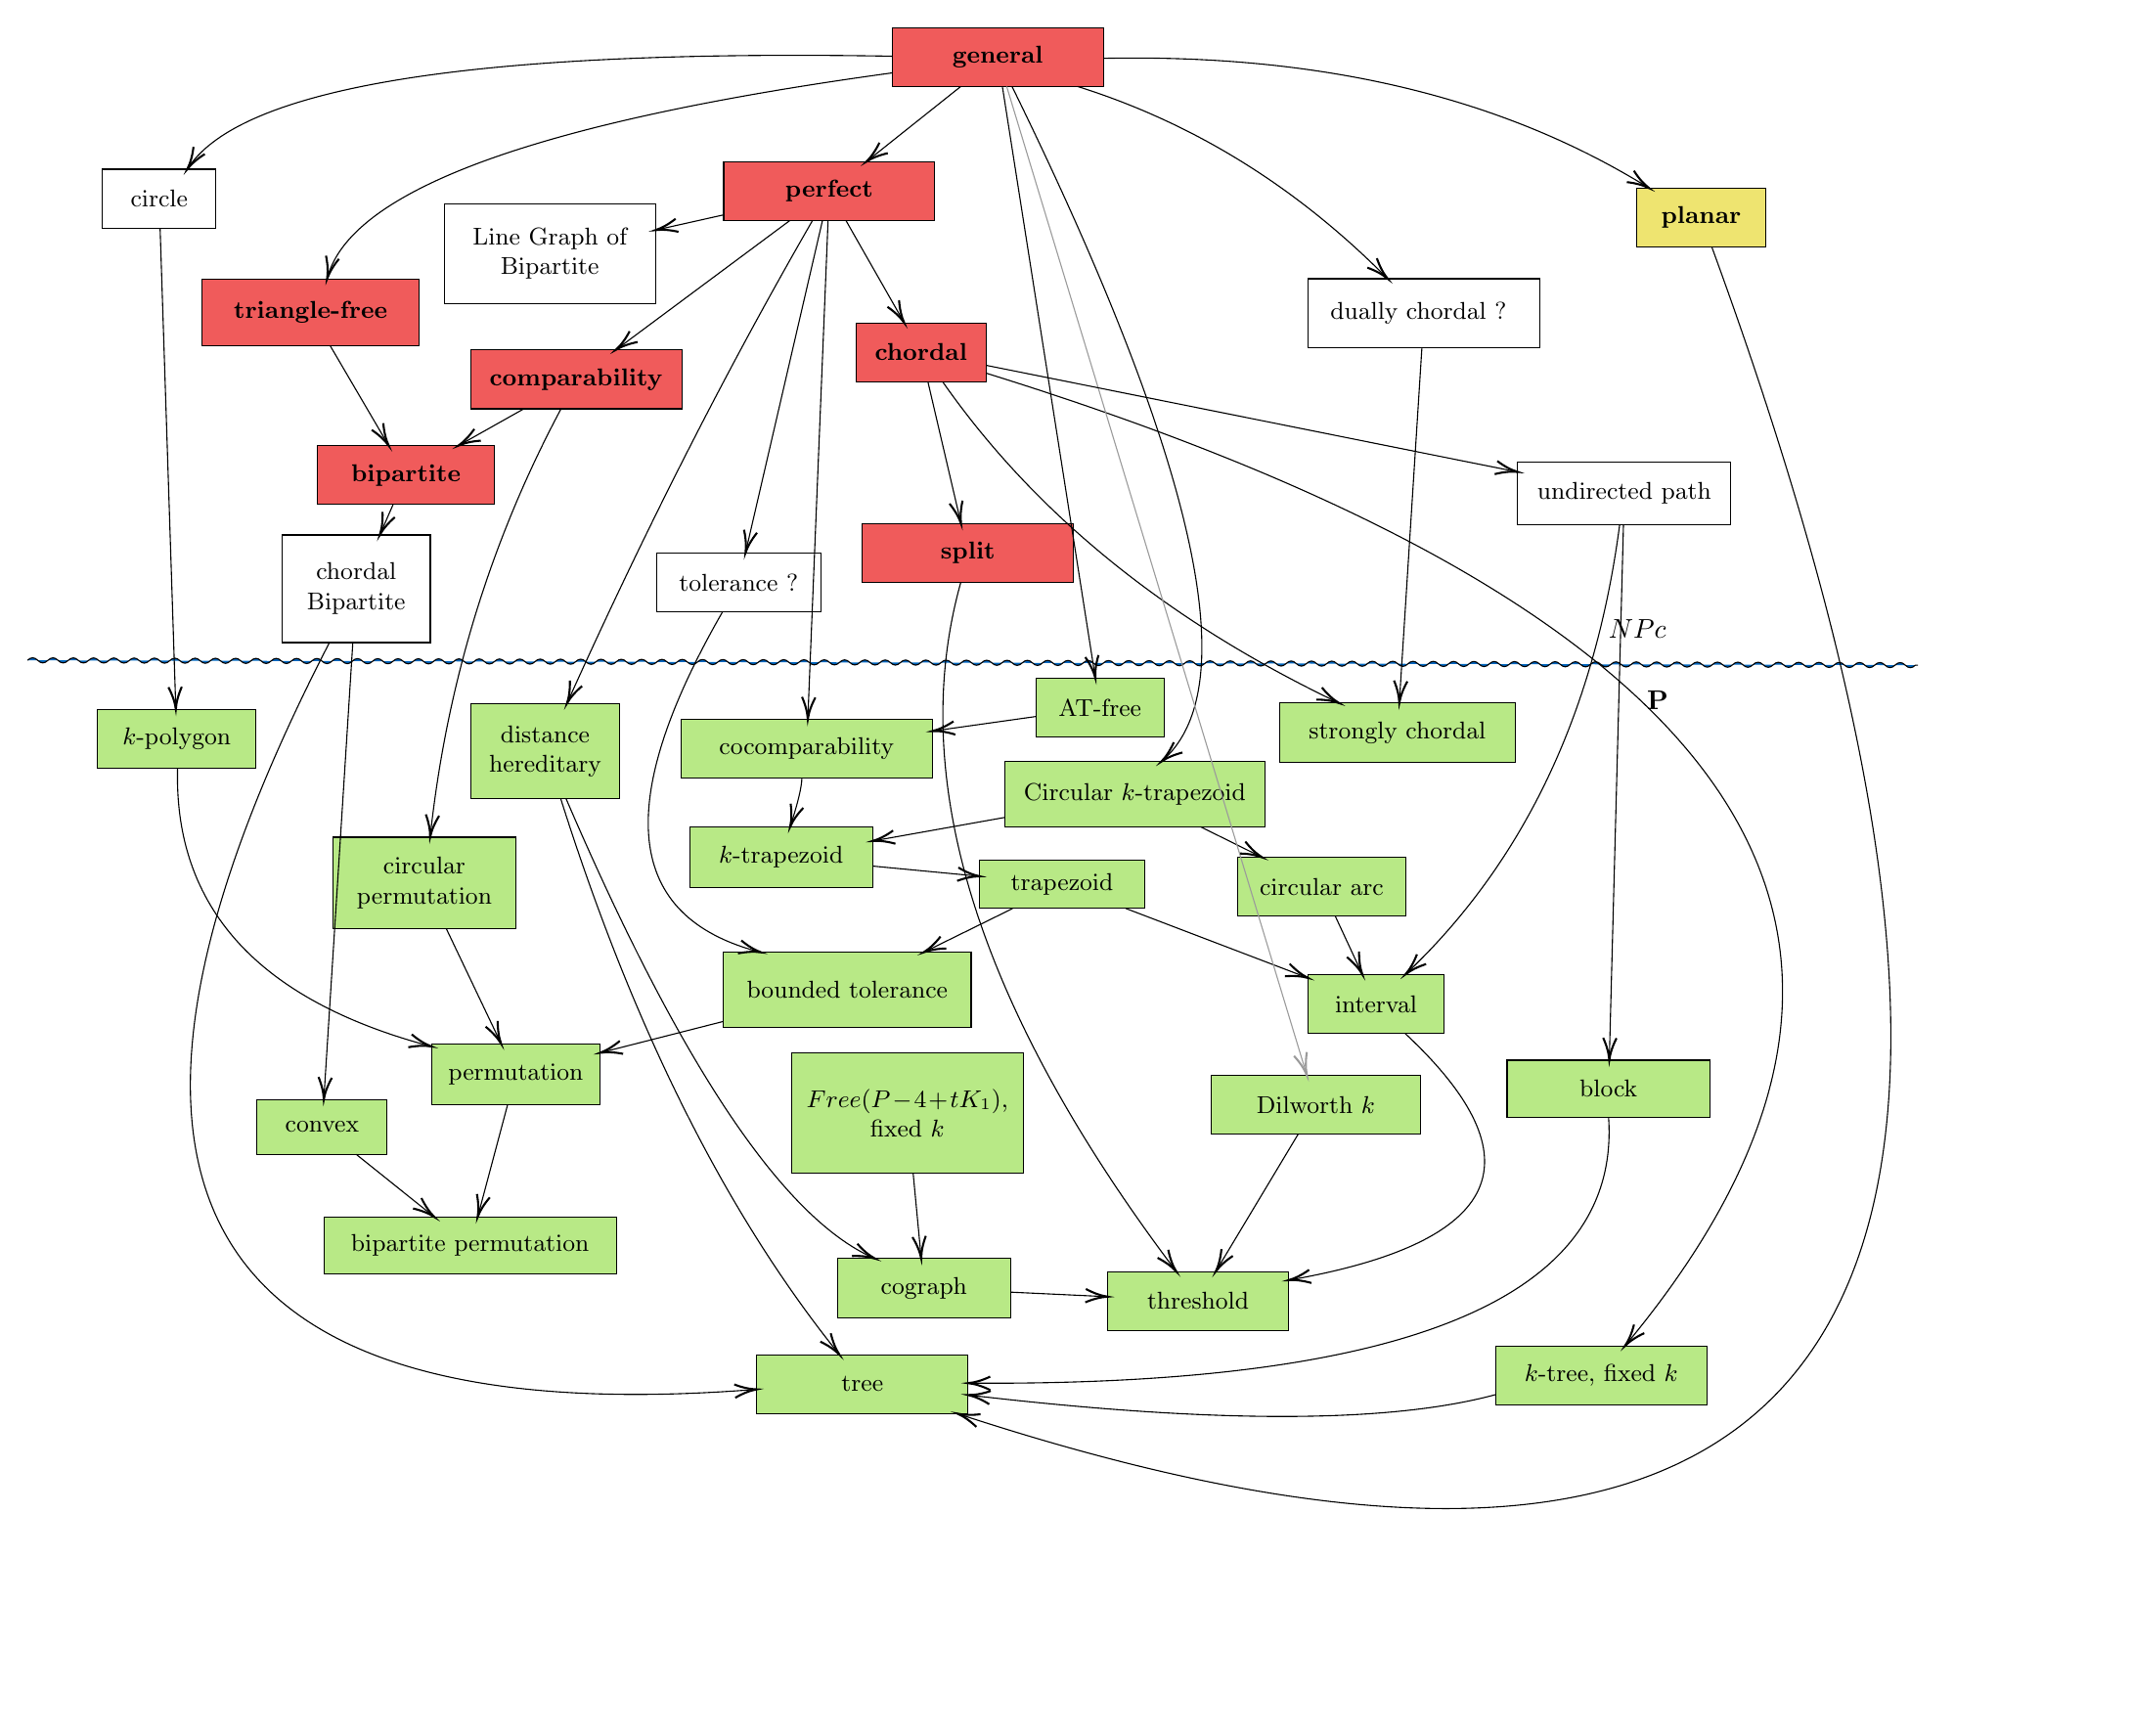
\begin{tikzpicture}[x=0.75pt,y=0.75pt,yscale=-1,xscale=1]
%uncomment if require: \path (0,617); %set diagram left start at 0, and has height of 617

%Straight Lines [id:da6521298779049807] 
\draw [fill={rgb, 255:red, 0; green, 101; blue, 189 }  ,fill opacity=1 ]   (-114.6,212.17) .. controls (-112.93,210.51) and (-111.26,210.52) .. (-109.6,212.19) .. controls (-107.93,213.86) and (-106.27,213.86) .. (-104.6,212.2) .. controls (-102.93,210.54) and (-101.27,210.54) .. (-99.6,212.21) .. controls (-97.94,213.88) and (-96.27,213.89) .. (-94.6,212.23) .. controls (-92.93,210.57) and (-91.27,210.57) .. (-89.6,212.24) .. controls (-87.93,213.91) and (-86.27,213.91) .. (-84.6,212.25) .. controls (-82.93,210.59) and (-81.26,210.6) .. (-79.6,212.27) .. controls (-77.93,213.94) and (-76.27,213.94) .. (-74.6,212.28) .. controls (-72.93,210.62) and (-71.27,210.62) .. (-69.6,212.29) .. controls (-67.93,213.96) and (-66.27,213.96) .. (-64.6,212.3) .. controls (-62.93,210.64) and (-61.26,210.65) .. (-59.6,212.32) .. controls (-57.93,213.99) and (-56.27,213.99) .. (-54.6,212.33) .. controls (-52.93,210.67) and (-51.27,210.67) .. (-49.6,212.34) .. controls (-47.94,214.01) and (-46.27,214.02) .. (-44.6,212.36) .. controls (-42.93,210.7) and (-41.27,210.7) .. (-39.6,212.37) .. controls (-37.93,214.04) and (-36.27,214.04) .. (-34.6,212.38) .. controls (-32.93,210.72) and (-31.27,210.72) .. (-29.6,212.39) .. controls (-27.94,214.06) and (-26.27,214.07) .. (-24.6,212.41) .. controls (-22.93,210.75) and (-21.27,210.75) .. (-19.6,212.42) .. controls (-17.93,214.09) and (-16.27,214.09) .. (-14.6,212.43) .. controls (-12.93,210.77) and (-11.26,210.78) .. (-9.6,212.45) .. controls (-7.93,214.12) and (-6.27,214.12) .. (-4.6,212.46) .. controls (-2.93,210.8) and (-1.27,210.8) .. (0.4,212.47) .. controls (2.07,214.14) and (3.73,214.14) .. (5.4,212.48) .. controls (7.07,210.82) and (8.74,210.83) .. (10.4,212.5) .. controls (12.07,214.17) and (13.73,214.17) .. (15.4,212.51) .. controls (17.07,210.85) and (18.73,210.85) .. (20.4,212.52) .. controls (22.06,214.19) and (23.73,214.2) .. (25.4,212.54) .. controls (27.07,210.88) and (28.73,210.88) .. (30.4,212.55) .. controls (32.07,214.22) and (33.73,214.22) .. (35.4,212.56) .. controls (37.07,210.9) and (38.73,210.9) .. (40.4,212.57) .. controls (42.06,214.24) and (43.73,214.25) .. (45.4,212.59) .. controls (47.07,210.93) and (48.73,210.93) .. (50.4,212.6) .. controls (52.07,214.27) and (53.73,214.27) .. (55.4,212.61) .. controls (57.07,210.95) and (58.74,210.96) .. (60.4,212.63) .. controls (62.07,214.3) and (63.73,214.3) .. (65.4,212.64) .. controls (67.07,210.98) and (68.73,210.98) .. (70.4,212.65) .. controls (72.07,214.32) and (73.73,214.32) .. (75.4,212.66) .. controls (77.07,211) and (78.74,211.01) .. (80.4,212.68) .. controls (82.07,214.35) and (83.73,214.35) .. (85.4,212.69) .. controls (87.07,211.03) and (88.73,211.03) .. (90.4,212.7) .. controls (92.06,214.37) and (93.73,214.38) .. (95.4,212.72) .. controls (97.07,211.06) and (98.73,211.06) .. (100.4,212.73) .. controls (102.07,214.4) and (103.73,214.4) .. (105.4,212.74) .. controls (107.07,211.08) and (108.73,211.08) .. (110.4,212.75) .. controls (112.06,214.42) and (113.73,214.43) .. (115.4,212.77) .. controls (117.07,211.11) and (118.73,211.11) .. (120.4,212.78) .. controls (122.07,214.45) and (123.73,214.45) .. (125.4,212.79) .. controls (127.07,211.13) and (128.74,211.14) .. (130.4,212.81) .. controls (132.07,214.48) and (133.73,214.48) .. (135.4,212.82) .. controls (137.07,211.16) and (138.73,211.16) .. (140.4,212.83) .. controls (142.06,214.5) and (143.73,214.51) .. (145.4,212.85) .. controls (147.07,211.19) and (148.73,211.19) .. (150.4,212.86) .. controls (152.07,214.53) and (153.73,214.53) .. (155.4,212.87) .. controls (157.07,211.21) and (158.73,211.21) .. (160.4,212.88) .. controls (162.06,214.55) and (163.73,214.56) .. (165.4,212.9) .. controls (167.07,211.24) and (168.73,211.24) .. (170.4,212.91) .. controls (172.07,214.58) and (173.73,214.58) .. (175.4,212.92) .. controls (177.07,211.26) and (178.74,211.27) .. (180.4,212.94) .. controls (182.07,214.61) and (183.73,214.61) .. (185.4,212.95) .. controls (187.07,211.29) and (188.73,211.29) .. (190.4,212.96) .. controls (192.07,214.63) and (193.73,214.63) .. (195.4,212.97) .. controls (197.07,211.31) and (198.74,211.32) .. (200.4,212.99) .. controls (202.07,214.66) and (203.73,214.66) .. (205.4,213) .. controls (207.07,211.34) and (208.73,211.34) .. (210.4,213.01) .. controls (212.06,214.68) and (213.73,214.69) .. (215.4,213.03) .. controls (217.07,211.37) and (218.73,211.37) .. (220.4,213.04) .. controls (222.07,214.71) and (223.73,214.71) .. (225.4,213.05) .. controls (227.07,211.39) and (228.73,211.39) .. (230.4,213.06) .. controls (232.06,214.73) and (233.73,214.74) .. (235.4,213.08) .. controls (237.07,211.42) and (238.73,211.42) .. (240.4,213.09) .. controls (242.07,214.76) and (243.73,214.76) .. (245.4,213.1) .. controls (247.07,211.44) and (248.74,211.45) .. (250.4,213.12) .. controls (252.07,214.79) and (253.73,214.79) .. (255.4,213.13) .. controls (257.07,211.47) and (258.73,211.47) .. (260.4,213.14) .. controls (262.07,214.81) and (263.73,214.81) .. (265.4,213.15) .. controls (267.07,211.49) and (268.74,211.5) .. (270.4,213.17) .. controls (272.07,214.84) and (273.73,214.84) .. (275.4,213.18) .. controls (277.07,211.52) and (278.73,211.52) .. (280.4,213.19) .. controls (282.06,214.86) and (283.73,214.87) .. (285.4,213.21) .. controls (287.07,211.55) and (288.73,211.55) .. (290.4,213.22) .. controls (292.07,214.89) and (293.73,214.89) .. (295.4,213.23) .. controls (297.07,211.57) and (298.73,211.57) .. (300.4,213.24) .. controls (302.06,214.91) and (303.73,214.92) .. (305.4,213.26) .. controls (307.07,211.6) and (308.73,211.6) .. (310.4,213.27) .. controls (312.07,214.94) and (313.73,214.94) .. (315.4,213.28) .. controls (317.07,211.62) and (318.74,211.63) .. (320.4,213.3) .. controls (322.07,214.97) and (323.73,214.97) .. (325.4,213.31) .. controls (327.07,211.65) and (328.73,211.65) .. (330.4,213.32) .. controls (332.07,214.99) and (333.73,214.99) .. (335.4,213.33) .. controls (337.07,211.67) and (338.74,211.68) .. (340.4,213.35) .. controls (342.07,215.02) and (343.73,215.02) .. (345.4,213.36) .. controls (347.07,211.7) and (348.73,211.7) .. (350.4,213.37) .. controls (352.06,215.04) and (353.73,215.05) .. (355.4,213.39) .. controls (357.07,211.73) and (358.73,211.73) .. (360.4,213.4) .. controls (362.07,215.07) and (363.73,215.07) .. (365.4,213.41) .. controls (367.07,211.75) and (368.73,211.75) .. (370.4,213.42) .. controls (372.06,215.09) and (373.73,215.1) .. (375.4,213.44) .. controls (377.07,211.78) and (378.73,211.78) .. (380.4,213.45) .. controls (382.07,215.12) and (383.73,215.12) .. (385.4,213.46) .. controls (387.07,211.8) and (388.74,211.81) .. (390.4,213.48) .. controls (392.07,215.15) and (393.73,215.15) .. (395.4,213.49) .. controls (397.07,211.83) and (398.73,211.83) .. (400.4,213.5) .. controls (402.06,215.17) and (403.73,215.18) .. (405.4,213.52) .. controls (407.07,211.86) and (408.73,211.86) .. (410.4,213.53) .. controls (412.07,215.2) and (413.73,215.2) .. (415.4,213.54) .. controls (417.07,211.88) and (418.73,211.88) .. (420.4,213.55) .. controls (422.06,215.22) and (423.73,215.23) .. (425.4,213.57) .. controls (427.07,211.91) and (428.73,211.91) .. (430.4,213.58) .. controls (432.07,215.25) and (433.73,215.25) .. (435.4,213.59) .. controls (437.07,211.93) and (438.74,211.94) .. (440.4,213.61) .. controls (442.07,215.28) and (443.73,215.28) .. (445.4,213.62) .. controls (447.07,211.96) and (448.73,211.96) .. (450.4,213.63) .. controls (452.07,215.3) and (453.73,215.3) .. (455.4,213.64) .. controls (457.07,211.98) and (458.74,211.99) .. (460.4,213.66) .. controls (462.07,215.33) and (463.73,215.33) .. (465.4,213.67) .. controls (467.07,212.01) and (468.73,212.01) .. (470.4,213.68) .. controls (472.06,215.35) and (473.73,215.36) .. (475.4,213.7) .. controls (477.07,212.04) and (478.73,212.04) .. (480.4,213.71) .. controls (482.07,215.38) and (483.73,215.38) .. (485.4,213.72) .. controls (487.07,212.06) and (488.73,212.06) .. (490.4,213.73) .. controls (492.06,215.4) and (493.73,215.41) .. (495.4,213.75) .. controls (497.07,212.09) and (498.73,212.09) .. (500.4,213.76) .. controls (502.07,215.43) and (503.73,215.43) .. (505.4,213.77) .. controls (507.07,212.11) and (508.74,212.12) .. (510.4,213.79) .. controls (512.07,215.46) and (513.73,215.46) .. (515.4,213.8) .. controls (517.07,212.14) and (518.73,212.14) .. (520.4,213.81) .. controls (522.07,215.48) and (523.73,215.48) .. (525.4,213.82) .. controls (527.07,212.16) and (528.74,212.17) .. (530.4,213.84) .. controls (532.07,215.51) and (533.73,215.51) .. (535.4,213.85) .. controls (537.07,212.19) and (538.73,212.19) .. (540.4,213.86) .. controls (542.06,215.53) and (543.73,215.54) .. (545.4,213.88) .. controls (547.07,212.22) and (548.73,212.22) .. (550.4,213.89) .. controls (552.07,215.56) and (553.73,215.56) .. (555.4,213.9) .. controls (557.07,212.24) and (558.73,212.24) .. (560.4,213.91) .. controls (562.06,215.58) and (563.73,215.59) .. (565.4,213.93) .. controls (567.07,212.27) and (568.73,212.27) .. (570.4,213.94) .. controls (572.07,215.61) and (573.73,215.61) .. (575.4,213.95) .. controls (577.07,212.29) and (578.74,212.3) .. (580.4,213.97) .. controls (582.07,215.64) and (583.73,215.64) .. (585.4,213.98) .. controls (587.07,212.32) and (588.73,212.32) .. (590.4,213.99) .. controls (592.07,215.66) and (593.73,215.66) .. (595.4,214) .. controls (597.07,212.34) and (598.74,212.35) .. (600.4,214.02) .. controls (602.07,215.69) and (603.73,215.69) .. (605.4,214.03) .. controls (607.07,212.37) and (608.73,212.37) .. (610.4,214.04) .. controls (612.06,215.71) and (613.73,215.72) .. (615.4,214.06) .. controls (617.07,212.4) and (618.73,212.4) .. (620.4,214.07) .. controls (622.07,215.74) and (623.73,215.74) .. (625.4,214.08) .. controls (627.07,212.42) and (628.74,212.43) .. (630.4,214.1) .. controls (632.07,215.77) and (633.73,215.77) .. (635.4,214.11) .. controls (637.07,212.45) and (638.73,212.45) .. (640.4,214.12) .. controls (642.07,215.79) and (643.73,215.79) .. (645.4,214.13) .. controls (647.07,212.47) and (648.74,212.48) .. (650.4,214.15) .. controls (652.07,215.82) and (653.73,215.82) .. (655.4,214.16) .. controls (657.07,212.5) and (658.73,212.5) .. (660.4,214.17) .. controls (662.06,215.84) and (663.73,215.85) .. (665.4,214.19) .. controls (667.07,212.53) and (668.73,212.53) .. (670.4,214.2) .. controls (672.07,215.87) and (673.73,215.87) .. (675.4,214.21) .. controls (677.07,212.55) and (678.73,212.55) .. (680.4,214.22) .. controls (682.06,215.89) and (683.73,215.9) .. (685.4,214.24) .. controls (687.07,212.58) and (688.73,212.58) .. (690.4,214.25) .. controls (692.07,215.92) and (693.73,215.92) .. (695.4,214.26) .. controls (697.07,212.6) and (698.74,212.61) .. (700.4,214.28) .. controls (702.07,215.95) and (703.73,215.95) .. (705.4,214.29) .. controls (707.07,212.63) and (708.73,212.63) .. (710.4,214.3) .. controls (712.07,215.97) and (713.73,215.97) .. (715.4,214.31) .. controls (717.07,212.65) and (718.74,212.66) .. (720.4,214.33) .. controls (722.07,216) and (723.73,216) .. (725.4,214.34) .. controls (727.07,212.68) and (728.73,212.68) .. (730.4,214.35) .. controls (732.06,216.02) and (733.73,216.03) .. (735.4,214.37) .. controls (737.07,212.71) and (738.73,212.71) .. (740.4,214.38) .. controls (742.07,216.05) and (743.73,216.05) .. (745.4,214.39) .. controls (747.07,212.73) and (748.73,212.73) .. (750.4,214.4) .. controls (752.06,216.07) and (753.73,216.08) .. (755.4,214.42) .. controls (757.07,212.76) and (758.73,212.76) .. (760.4,214.43) .. controls (762.07,216.1) and (763.73,216.1) .. (765.4,214.44) .. controls (767.07,212.78) and (768.74,212.79) .. (770.4,214.46) .. controls (772.07,216.13) and (773.73,216.13) .. (775.4,214.47) .. controls (777.07,212.81) and (778.73,212.81) .. (780.4,214.48) .. controls (782.07,216.15) and (783.73,216.15) .. (785.4,214.49) .. controls (787.07,212.83) and (788.74,212.84) .. (790.4,214.51) .. controls (792.07,216.18) and (793.73,216.18) .. (795.4,214.52) .. controls (797.07,212.86) and (798.73,212.86) .. (800.4,214.53) .. controls (802.06,216.2) and (803.73,216.21) .. (805.4,214.55) .. controls (807.07,212.89) and (808.73,212.89) .. (810.4,214.56) .. controls (812.07,216.23) and (813.73,216.23) .. (815.4,214.57) -- (816.6,214.57) -- (816.6,214.57) ;

% Text Node
\draw  [fill={rgb, 255:red, 233; green, 17; blue, 17 }  ,fill opacity=0.69 ]  (228.33,-33.4) -- (332.33,-33.4) -- (332.33,-4.4) -- (228.33,-4.4) -- cycle  ;
\draw (280.33,-18.9) node  [font=\small] [align=left] {\begin{minipage}[lt]{68pt}\setlength\topsep{0pt}
\begin{center}
\textbf{perfect}
\end{center}

\end{minipage}};
% Text Node
\draw    (90.67,-12.58) -- (194.67,-12.58) -- (194.67,36.42) -- (90.67,36.42) -- cycle  ;
\draw (142.67,11.92) node  [font=\small] [align=left] {\begin{minipage}[lt]{68pt}\setlength\topsep{0pt}
\begin{center}
Line Graph of Bipartite
\end{center}

\end{minipage}};
% Text Node
\draw  [fill={rgb, 255:red, 233; green, 17; blue, 17 }  ,fill opacity=0.69 ]  (103.67,59.27) -- (207.67,59.27) -- (207.67,88.27) -- (103.67,88.27) -- cycle  ;
\draw (155.67,73.77) node  [font=\small] [align=left] {\begin{minipage}[lt]{68pt}\setlength\topsep{0pt}
\begin{center}
\textbf{comparability}
\end{center}

\end{minipage}};
% Text Node
\draw    (195.2,159.27) -- (276.2,159.27) -- (276.2,188.27) -- (195.2,188.27) -- cycle  ;
\draw (235.7,173.77) node  [font=\small] [align=left] {\begin{minipage}[lt]{52.63pt}\setlength\topsep{0pt}
\begin{center}
tolerance ?
\end{center}

\end{minipage}};
% Text Node
\draw  [fill={rgb, 255:red, 184; green, 233; blue, 134 }  ,fill opacity=1 ]  (382.2,220.93) -- (445.2,220.93) -- (445.2,249.93) -- (382.2,249.93) -- cycle  ;
\draw (413.7,235.43) node  [font=\small] [align=left] {\begin{minipage}[lt]{40.39pt}\setlength\topsep{0pt}
\begin{center}
AT-free
\end{center}

\end{minipage}};
% Text Node
\draw  [fill={rgb, 255:red, 233; green, 17; blue, 17 }  ,fill opacity=0.69 ]  (293.53,45.93) -- (357.53,45.93) -- (357.53,74.93) -- (293.53,74.93) -- cycle  ;
\draw (325.53,60.43) node  [font=\small] [align=left] {\begin{minipage}[lt]{40.62pt}\setlength\topsep{0pt}
\begin{center}
\textbf{chordal}
\end{center}

\end{minipage}};
% Text Node
\draw  [fill={rgb, 255:red, 233; green, 17; blue, 17 }  ,fill opacity=0.69 ]  (296.67,144.93) -- (400.67,144.93) -- (400.67,173.93) -- (296.67,173.93) -- cycle  ;
\draw (348.67,159.43) node  [font=\small] [align=left] {\begin{minipage}[lt]{68pt}\setlength\topsep{0pt}
\begin{center}
\textbf{split}
\end{center}

\end{minipage}};
% Text Node
\draw  [fill={rgb, 255:red, 184; green, 233; blue, 134 }  ,fill opacity=1 ]  (608.67,549.93) -- (712.67,549.93) -- (712.67,578.93) -- (608.67,578.93) -- cycle  ;
\draw (660.67,564.43) node  [font=\small] [align=left] {\begin{minipage}[lt]{68pt}\setlength\topsep{0pt}
\begin{center}
$\displaystyle k$-tree, fixed $\displaystyle k$
\end{center}

\end{minipage}};
% Text Node
\draw  [color={rgb, 255:red, 0; green, 0; blue, 0 }  ,draw opacity=1 ][fill={rgb, 255:red, 184; green, 233; blue, 134 }  ,fill opacity=1 ]  (207.17,241.27) -- (331.17,241.27) -- (331.17,270.27) -- (207.17,270.27) -- cycle  ;
\draw (269.17,255.77) node  [font=\small] [align=left] {\begin{minipage}[lt]{81.83pt}\setlength\topsep{0pt}
\begin{center}
cocomparability
\end{center}

\end{minipage}};
% Text Node
\draw  [fill={rgb, 255:red, 184; green, 233; blue, 134 }  ,fill opacity=1 ]  (244.67,554.27) -- (348.67,554.27) -- (348.67,583.27) -- (244.67,583.27) -- cycle  ;
\draw (296.67,568.77) node  [font=\small] [align=left] {\begin{minipage}[lt]{68pt}\setlength\topsep{0pt}
\begin{center}
tree
\end{center}

\end{minipage}};
% Text Node
\draw    (-77.8,-29.73) -- (-21.8,-29.73) -- (-21.8,-0.73) -- (-77.8,-0.73) -- cycle  ;
\draw (-49.8,-15.23) node  [font=\small] [align=left] {\begin{minipage}[lt]{35.63pt}\setlength\topsep{0pt}
\begin{center}
circle
\end{center}

\end{minipage}};
% Text Node
\draw    (10.8,150.42) -- (83.8,150.42) -- (83.8,203.42) -- (10.8,203.42) -- cycle  ;
\draw (47.3,176.92) node  [font=\small] [align=left] {\begin{minipage}[lt]{47.1pt}\setlength\topsep{0pt}
\begin{center}
chordal Bipartite
\end{center}

\end{minipage}};
% Text Node
\draw  [fill={rgb, 255:red, 233; green, 17; blue, 17 }  ,fill opacity=0.69 ]  (28.3,106.47) -- (115.3,106.47) -- (115.3,135.47) -- (28.3,135.47) -- cycle  ;
\draw (71.8,120.97) node  [font=\small] [align=left] {\begin{minipage}[lt]{56.39pt}\setlength\topsep{0pt}
\begin{center}
\textbf{bipartite}
\end{center}

\end{minipage}};
% Text Node
\draw  [fill={rgb, 255:red, 184; green, 233; blue, 134 }  ,fill opacity=1 ]  (366.87,262.15) -- (494.87,262.15) -- (494.87,294.15) -- (366.87,294.15) -- cycle  ;
\draw (430.87,278.15) node  [font=\small] [align=left] {\begin{minipage}[lt]{84.59pt}\setlength\topsep{0pt}
\begin{center}
Circular $\displaystyle k$-trapezoid
\end{center}

\end{minipage}};
% Text Node
\draw  [fill={rgb, 255:red, 184; green, 233; blue, 134 }  ,fill opacity=1 ]  (211.6,294.24) -- (301.6,294.24) -- (301.6,324.24) -- (211.6,324.24) -- cycle  ;
\draw (256.6,309.24) node  [font=\small] [align=left] {\begin{minipage}[lt]{58.21pt}\setlength\topsep{0pt}
\begin{center}
$\displaystyle k$-trapezoid
\end{center}

\end{minipage}};
% Text Node
\draw  [fill={rgb, 255:red, 184; green, 233; blue, 134 }  ,fill opacity=1 ]  (354.53,310.45) -- (435.53,310.45) -- (435.53,334.45) -- (354.53,334.45) -- cycle  ;
\draw (395.03,322.45) node  [font=\small] [align=left] {\begin{minipage}[lt]{52.18pt}\setlength\topsep{0pt}
\begin{center}
trapezoid
\end{center}

\end{minipage}};
% Text Node
\draw  [fill={rgb, 255:red, 184; green, 233; blue, 134 }  ,fill opacity=1 ]  (228.2,356.05) -- (350.2,356.05) -- (350.2,393.05) -- (228.2,393.05) -- cycle  ;
\draw (289.2,374.55) node  [font=\small] [align=left] {\begin{minipage}[lt]{80.51pt}\setlength\topsep{0pt}
\begin{center}
bounded tolerance
\end{center}

\end{minipage}};
% Text Node
\draw  [fill={rgb, 255:red, 184; green, 233; blue, 134 }  ,fill opacity=1 ]  (84.37,401.11) -- (167.37,401.11) -- (167.37,431.11) -- (84.37,431.11) -- cycle  ;
\draw (125.87,416.11) node  [font=\small] [align=left] {\begin{minipage}[lt]{53.77pt}\setlength\topsep{0pt}
\begin{center}
permutation
\end{center}

\end{minipage}};
% Text Node
\draw  [fill={rgb, 255:red, 184; green, 233; blue, 134 }  ,fill opacity=1 ]  (31.37,486.49) -- (175.37,486.49) -- (175.37,514.49) -- (31.37,514.49) -- cycle  ;
\draw (103.37,500.49) node  [font=\small] [align=left] {\begin{minipage}[lt]{95.25pt}\setlength\topsep{0pt}
\begin{center}
bipartite permutation
\end{center}

\end{minipage}};
% Text Node
\draw  [fill={rgb, 255:red, 184; green, 233; blue, 134 }  ,fill opacity=1 ]  (-1.53,428.57) -- (62.47,428.57) -- (62.47,455.57) -- (-1.53,455.57) -- cycle  ;
\draw (30.47,442.07) node  [font=\small] [align=left] {\begin{minipage}[lt]{40.53pt}\setlength\topsep{0pt}
\begin{center}
convex
\end{center}

\end{minipage}};
% Text Node
\draw  [fill={rgb, 255:red, 184; green, 233; blue, 134 }  ,fill opacity=1 ]  (516.2,366.93) -- (583.2,366.93) -- (583.2,395.93) -- (516.2,395.93) -- cycle  ;
\draw (549.7,381.43) node  [font=\small] [align=left] {\begin{minipage}[lt]{43.11pt}\setlength\topsep{0pt}
\begin{center}
interval
\end{center}

\end{minipage}};
% Text Node
\draw  [fill={rgb, 255:red, 184; green, 233; blue, 134 }  ,fill opacity=1 ]  (417.53,513.27) -- (506.53,513.27) -- (506.53,542.27) -- (417.53,542.27) -- cycle  ;
\draw (462.03,527.77) node  [font=\small] [align=left] {\begin{minipage}[lt]{57.62pt}\setlength\topsep{0pt}
\begin{center}
threshold
\end{center}

\end{minipage}};
% Text Node
\draw  [fill={rgb, 255:red, 184; green, 233; blue, 134 }  ,fill opacity=1 ]  (468.53,416.6) -- (571.53,416.6) -- (571.53,445.6) -- (468.53,445.6) -- cycle  ;
\draw (520.03,431.1) node  [font=\small] [align=left] {\begin{minipage}[lt]{67.14pt}\setlength\topsep{0pt}
\begin{center}
Dilworth $\displaystyle k$
\end{center}

\end{minipage}};
% Text Node
\draw  [fill={rgb, 255:red, 184; green, 233; blue, 134 }  ,fill opacity=1 ]  (284.53,506.93) -- (369.53,506.93) -- (369.53,535.93) -- (284.53,535.93) -- cycle  ;
\draw (327.03,521.43) node  [font=\small] [align=left] {\begin{minipage}[lt]{55.35pt}\setlength\topsep{0pt}
\begin{center}
cograph
\end{center}

\end{minipage}};
% Text Node
\draw  [fill={rgb, 255:red, 184; green, 233; blue, 134 }  ,fill opacity=1 ]  (481.4,309.27) -- (564.4,309.27) -- (564.4,338.27) -- (481.4,338.27) -- cycle  ;
\draw (522.9,323.77) node  [font=\small] [align=left] {\begin{minipage}[lt]{53.72pt}\setlength\topsep{0pt}
\begin{center}
circular arc
\end{center}

\end{minipage}};
% Text Node
\draw  [fill={rgb, 255:red, 255; green, 255; blue, 255 }  ,fill opacity=1 ]  (516.37,24.22) -- (630.37,24.22) -- (630.37,58.22) -- (516.37,58.22) -- cycle  ;
\draw (573.37,41.22) node  [font=\small] [align=left] {\begin{minipage}[lt]{74.85pt}\setlength\topsep{0pt}
\begin{center}
dually chordal ? $ $
\end{center}

\end{minipage}};
% Text Node
\draw  [fill={rgb, 255:red, 184; green, 233; blue, 134 }  ,fill opacity=1 ]  (502.23,233.27) -- (618.23,233.27) -- (618.23,262.27) -- (502.23,262.27) -- cycle  ;
\draw (560.23,247.77) node  [font=\small] [align=left] {\begin{minipage}[lt]{76.39pt}\setlength\topsep{0pt}
\begin{center}
strongly chordal
\end{center}

\end{minipage}};
% Text Node
\draw  [fill={rgb, 255:red, 184; green, 233; blue, 134 }  ,fill opacity=1 ]  (35.9,299.3) -- (125.9,299.3) -- (125.9,344.3) -- (35.9,344.3) -- cycle  ;
\draw (80.9,321.8) node  [font=\small] [align=left] {\begin{minipage}[lt]{58.34pt}\setlength\topsep{0pt}
\begin{center}
circular permutation
\end{center}

\end{minipage}};
% Text Node
\draw  [fill={rgb, 255:red, 184; green, 233; blue, 134 }  ,fill opacity=1 ]  (-80.1,236.27) -- (-2.1,236.27) -- (-2.1,265.27) -- (-80.1,265.27) -- cycle  ;
\draw (-41.1,250.77) node  [font=\small] [align=left] {\begin{minipage}[lt]{50.18pt}\setlength\topsep{0pt}
\begin{center}
$\displaystyle k$-polygon
\end{center}

\end{minipage}};
% Text Node
\draw  [fill={rgb, 255:red, 184; green, 233; blue, 134 }  ,fill opacity=1 ]  (103.9,233.49) -- (176.9,233.49) -- (176.9,280.49) -- (103.9,280.49) -- cycle  ;
\draw (140.4,256.99) node  [font=\small] [align=left] {\begin{minipage}[lt]{46.78pt}\setlength\topsep{0pt}
\begin{center}
distance hereditary
\end{center}

\end{minipage}};
% Text Node
\draw  [fill={rgb, 255:red, 184; green, 233; blue, 134 }  ,fill opacity=1 ]  (261.83,405.74) -- (375.83,405.74) -- (375.83,464.74) -- (261.83,464.74) -- cycle  ;
\draw (318.83,435.24) node  [font=\small] [align=left] {\begin{minipage}[lt]{74.57pt}\setlength\topsep{0pt}
\begin{center}
$\displaystyle Free( P-4+tK_{1})$, fixed $\displaystyle k$
\end{center}

\end{minipage}};
% Text Node
\draw  [fill={rgb, 255:red, 230; green, 216; blue, 48 }  ,fill opacity=0.69 ]  (677.87,-20.4) -- (741.87,-20.4) -- (741.87,8.6) -- (677.87,8.6) -- cycle  ;
\draw (709.87,-5.9) node  [font=\small] [align=left] {\begin{minipage}[lt]{40.62pt}\setlength\topsep{0pt}
\begin{center}
\textbf{planar}
\end{center}

\end{minipage}};
% Text Node
\draw (663,191) node [anchor=north west][inner sep=0.75pt]   [align=left] {$\displaystyle NPc$};
% Text Node
\draw (682,226) node [anchor=north west][inner sep=0.75pt]   [align=left] {\textbf{P}};
% Text Node
\draw  [fill={rgb, 255:red, 233; green, 17; blue, 17 }  ,fill opacity=0.69 ]  (311.33,-99.5) -- (415.33,-99.5) -- (415.33,-70.5) -- (311.33,-70.5) -- cycle  ;
\draw (363.33,-85) node  [font=\small] [align=left] {\begin{minipage}[lt]{68pt}\setlength\topsep{0pt}
\begin{center}
\textbf{general}
\end{center}

\end{minipage}};
% Text Node
\draw  [fill={rgb, 255:red, 184; green, 233; blue, 134 }  ,fill opacity=1 ]  (614.23,409.17) -- (714.23,409.17) -- (714.23,437.17) -- (614.23,437.17) -- cycle  ;
\draw (664.23,423.17) node  [font=\small] [align=left] {\begin{minipage}[lt]{65.51pt}\setlength\topsep{0pt}
\begin{center}
block
\end{center}

\end{minipage}};
% Text Node
\draw  [fill={rgb, 255:red, 255; green, 255; blue, 255 }  ,fill opacity=1 ]  (619.5,114.42) -- (724.5,114.42) -- (724.5,145.42) -- (619.5,145.42) -- cycle  ;
\draw (672,129.92) node  [font=\small] [align=left] {\begin{minipage}[lt]{68.82pt}\setlength\topsep{0pt}
\begin{center}
undirected path
\end{center}

\end{minipage}};
% Text Node
\draw  [fill={rgb, 255:red, 233; green, 17; blue, 17 }  ,fill opacity=0.69 ]  (-28.67,24.26) -- (78.33,24.26) -- (78.33,57.26) -- (-28.67,57.26) -- cycle  ;
\draw (24.83,40.76) node  [font=\small] [align=left] {\begin{minipage}[lt]{69.95pt}\setlength\topsep{0pt}
\begin{center}
\textbf{triangle-free}
\end{center}

\end{minipage}};
% Connection
\draw    (260.83,-4.4) -- (176.78,58.07) ;
\draw [shift={(175.17,59.27)}, rotate = 323.38] [color={rgb, 255:red, 0; green, 0; blue, 0 }  ][line width=0.75]    (10.93,-3.29) .. controls (6.95,-1.4) and (3.31,-0.3) .. (0,0) .. controls (3.31,0.3) and (6.95,1.4) .. (10.93,3.29)   ;
% Connection
\draw    (276.97,-4.4) -- (239.51,157.32) ;
\draw [shift={(239.06,159.27)}, rotate = 283.04] [color={rgb, 255:red, 0; green, 0; blue, 0 }  ][line width=0.75]    (10.93,-3.29) .. controls (6.95,-1.4) and (3.31,-0.3) .. (0,0) .. controls (3.31,0.3) and (6.95,1.4) .. (10.93,3.29)   ;
% Connection
\draw    (288.59,-4.4) -- (316.28,44.2) ;
\draw [shift={(317.27,45.93)}, rotate = 240.33] [color={rgb, 255:red, 0; green, 0; blue, 0 }  ][line width=0.75]    (10.93,-3.29) .. controls (6.95,-1.4) and (3.31,-0.3) .. (0,0) .. controls (3.31,0.3) and (6.95,1.4) .. (10.93,3.29)   ;
% Connection
\draw    (328.92,74.93) -- (344.82,142.99) ;
\draw [shift={(345.28,144.93)}, rotate = 256.85] [color={rgb, 255:red, 0; green, 0; blue, 0 }  ][line width=0.75]    (10.93,-3.29) .. controls (6.95,-1.4) and (3.31,-0.3) .. (0,0) .. controls (3.31,0.3) and (6.95,1.4) .. (10.93,3.29)   ;
% Connection
\draw    (357.53,70.7) .. controls (735.51,188.21) and (840.44,347.96) .. (672.32,549.93) ;
\draw [shift={(672.32,549.93)}, rotate = 309.77] [color={rgb, 255:red, 0; green, 0; blue, 0 }  ][line width=0.75]    (10.93,-3.29) .. controls (6.95,-1.4) and (3.31,-0.3) .. (0,0) .. controls (3.31,0.3) and (6.95,1.4) .. (10.93,3.29)   ;
% Connection
\draw    (382.2,239.86) -- (333.15,246.77) ;
\draw [shift={(331.17,247.04)}, rotate = 351.99] [color={rgb, 255:red, 0; green, 0; blue, 0 }  ][line width=0.75]    (10.93,-3.29) .. controls (6.95,-1.4) and (3.31,-0.3) .. (0,0) .. controls (3.31,0.3) and (6.95,1.4) .. (10.93,3.29)   ;
% Connection
\draw    (608.67,573.9) .. controls (556.14,588.12) and (470.09,588.26) .. (350.47,574.31) ;
\draw [shift={(348.67,574.1)}, rotate = 6.7] [color={rgb, 255:red, 0; green, 0; blue, 0 }  ][line width=0.75]    (10.93,-3.29) .. controls (6.95,-1.4) and (3.31,-0.3) .. (0,0) .. controls (3.31,0.3) and (6.95,1.4) .. (10.93,3.29)   ;
% Connection
\draw    (129.91,88.27) -- (99.3,105.49) ;
\draw [shift={(97.56,106.47)}, rotate = 330.62] [color={rgb, 255:red, 0; green, 0; blue, 0 }  ][line width=0.75]    (10.93,-3.29) .. controls (6.95,-1.4) and (3.31,-0.3) .. (0,0) .. controls (3.31,0.3) and (6.95,1.4) .. (10.93,3.29)   ;
% Connection
\draw    (65.45,135.47) -- (59.71,148.59) ;
\draw [shift={(58.9,150.42)}, rotate = 293.65] [color={rgb, 255:red, 0; green, 0; blue, 0 }  ][line width=0.75]    (10.93,-3.29) .. controls (6.95,-1.4) and (3.31,-0.3) .. (0,0) .. controls (3.31,0.3) and (6.95,1.4) .. (10.93,3.29)   ;
% Connection
\draw    (228.33,-7.26) -- (196.62,-0.16) ;
\draw [shift={(194.67,0.28)}, rotate = 347.38] [color={rgb, 255:red, 0; green, 0; blue, 0 }  ][line width=0.75]    (10.93,-3.29) .. controls (6.95,-1.4) and (3.31,-0.3) .. (0,0) .. controls (3.31,0.3) and (6.95,1.4) .. (10.93,3.29)   ;
% Connection
\draw    (366.87,289.57) -- (303.57,300.86) ;
\draw [shift={(301.6,301.21)}, rotate = 349.89] [color={rgb, 255:red, 0; green, 0; blue, 0 }  ][line width=0.75]    (10.93,-3.29) .. controls (6.95,-1.4) and (3.31,-0.3) .. (0,0) .. controls (3.31,0.3) and (6.95,1.4) .. (10.93,3.29)   ;
% Connection
\draw    (266.84,270.27) .. controls (266.74,274.5) and (265.01,281.87) .. (261.65,292.38) ;
\draw [shift={(261.04,294.24)}, rotate = 288.08] [color={rgb, 255:red, 0; green, 0; blue, 0 }  ][line width=0.75]    (10.93,-3.29) .. controls (6.95,-1.4) and (3.31,-0.3) .. (0,0) .. controls (3.31,0.3) and (6.95,1.4) .. (10.93,3.29)   ;
% Connection
\draw    (301.6,313.54) -- (352.54,318.4) ;
\draw [shift={(354.53,318.59)}, rotate = 185.45] [color={rgb, 255:red, 0; green, 0; blue, 0 }  ][line width=0.75]    (10.93,-3.29) .. controls (6.95,-1.4) and (3.31,-0.3) .. (0,0) .. controls (3.31,0.3) and (6.95,1.4) .. (10.93,3.29)   ;
% Connection
\draw    (370.66,334.45) -- (328.57,355.17) ;
\draw [shift={(326.78,356.05)}, rotate = 333.79] [color={rgb, 255:red, 0; green, 0; blue, 0 }  ][line width=0.75]    (10.93,-3.29) .. controls (6.95,-1.4) and (3.31,-0.3) .. (0,0) .. controls (3.31,0.3) and (6.95,1.4) .. (10.93,3.29)   ;
% Connection
\draw    (45.62,203.42) -- (31.45,426.58) ;
\draw [shift={(31.32,428.57)}, rotate = 273.63] [color={rgb, 255:red, 0; green, 0; blue, 0 }  ][line width=0.75]    (10.93,-3.29) .. controls (6.95,-1.4) and (3.31,-0.3) .. (0,0) .. controls (3.31,0.3) and (6.95,1.4) .. (10.93,3.29)   ;
% Connection
\draw [color={rgb, 255:red, 0; green, 0; blue, 0 }  ,draw opacity=1 ]   (47.31,455.57) -- (84.33,485.24) ;
\draw [shift={(85.89,486.49)}, rotate = 218.7] [color={rgb, 255:red, 0; green, 0; blue, 0 }  ,draw opacity=1 ][line width=0.75]    (10.93,-3.29) .. controls (6.95,-1.4) and (3.31,-0.3) .. (0,0) .. controls (3.31,0.3) and (6.95,1.4) .. (10.93,3.29)   ;
% Connection
\draw    (121.87,431.11) -- (107.62,484.56) ;
\draw [shift={(107.1,486.49)}, rotate = 284.93] [color={rgb, 255:red, 0; green, 0; blue, 0 }  ][line width=0.75]    (10.93,-3.29) .. controls (6.95,-1.4) and (3.31,-0.3) .. (0,0) .. controls (3.31,0.3) and (6.95,1.4) .. (10.93,3.29)   ;
% Connection
\draw    (228.2,390.07) -- (169.3,405.06) ;
\draw [shift={(167.37,405.55)}, rotate = 345.73] [color={rgb, 255:red, 0; green, 0; blue, 0 }  ][line width=0.75]    (10.93,-3.29) .. controls (6.95,-1.4) and (3.31,-0.3) .. (0,0) .. controls (3.31,0.3) and (6.95,1.4) .. (10.93,3.29)   ;
% Connection
\draw    (426.5,334.45) -- (514.33,367.95) ;
\draw [shift={(516.2,368.66)}, rotate = 200.87] [color={rgb, 255:red, 0; green, 0; blue, 0 }  ][line width=0.75]    (10.93,-3.29) .. controls (6.95,-1.4) and (3.31,-0.3) .. (0,0) .. controls (3.31,0.3) and (6.95,1.4) .. (10.93,3.29)   ;
% Connection
\draw    (563.94,395.93) .. controls (630.81,458.31) and (612.21,498.75) .. (508.11,517.28) ;
\draw [shift={(506.53,517.55)}, rotate = 350.11] [color={rgb, 255:red, 0; green, 0; blue, 0 }  ][line width=0.75]    (10.93,-3.29) .. controls (6.95,-1.4) and (3.31,-0.3) .. (0,0) .. controls (3.31,0.3) and (6.95,1.4) .. (10.93,3.29)   ;
% Connection
\draw    (369.53,523.43) -- (415.54,525.59) ;
\draw [shift={(417.53,525.68)}, rotate = 182.69] [color={rgb, 255:red, 0; green, 0; blue, 0 }  ][line width=0.75]    (10.93,-3.29) .. controls (6.95,-1.4) and (3.31,-0.3) .. (0,0) .. controls (3.31,0.3) and (6.95,1.4) .. (10.93,3.29)   ;
% Connection
\draw    (511.33,445.6) -- (471.76,511.55) ;
\draw [shift={(470.73,513.27)}, rotate = 300.96] [color={rgb, 255:red, 0; green, 0; blue, 0 }  ][line width=0.75]    (10.93,-3.29) .. controls (6.95,-1.4) and (3.31,-0.3) .. (0,0) .. controls (3.31,0.3) and (6.95,1.4) .. (10.93,3.29)   ;
% Connection
\draw    (345.09,173.93) .. controls (318.03,270.62) and (353.43,383.73) .. (451.29,513.27) ;
\draw [shift={(451.29,513.27)}, rotate = 232.93] [color={rgb, 255:red, 0; green, 0; blue, 0 }  ][line width=0.75]    (10.93,-3.29) .. controls (6.95,-1.4) and (3.31,-0.3) .. (0,0) .. controls (3.31,0.3) and (6.95,1.4) .. (10.93,3.29)   ;
% Connection
\draw    (529.64,338.27) -- (542.12,365.12) ;
\draw [shift={(542.96,366.93)}, rotate = 245.07] [color={rgb, 255:red, 0; green, 0; blue, 0 }  ][line width=0.75]    (10.93,-3.29) .. controls (6.95,-1.4) and (3.31,-0.3) .. (0,0) .. controls (3.31,0.3) and (6.95,1.4) .. (10.93,3.29)   ;
% Connection
\draw    (463.15,294.15) -- (491.85,308.38) ;
\draw [shift={(493.64,309.27)}, rotate = 206.36] [color={rgb, 255:red, 0; green, 0; blue, 0 }  ][line width=0.75]    (10.93,-3.29) .. controls (6.95,-1.4) and (3.31,-0.3) .. (0,0) .. controls (3.31,0.3) and (6.95,1.4) .. (10.93,3.29)   ;
% Connection
\draw    (572.29,58.22) -- (561.28,231.27) ;
\draw [shift={(561.16,233.27)}, rotate = 273.64] [color={rgb, 255:red, 0; green, 0; blue, 0 }  ][line width=0.75]    (10.93,-3.29) .. controls (6.95,-1.4) and (3.31,-0.3) .. (0,0) .. controls (3.31,0.3) and (6.95,1.4) .. (10.93,3.29)   ;
% Connection
\draw    (148.2,88.27) .. controls (113.41,153.53) and (91.96,223.51) .. (83.83,298.17) ;
\draw [shift={(83.71,299.3)}, rotate = 276.11] [color={rgb, 255:red, 0; green, 0; blue, 0 }  ][line width=0.75]    (10.93,-3.29) .. controls (6.95,-1.4) and (3.31,-0.3) .. (0,0) .. controls (3.31,0.3) and (6.95,1.4) .. (10.93,3.29)   ;
% Connection
\draw    (91.63,344.3) -- (117.85,399.3) ;
\draw [shift={(118.71,401.11)}, rotate = 244.51] [color={rgb, 255:red, 0; green, 0; blue, 0 }  ][line width=0.75]    (10.93,-3.29) .. controls (6.95,-1.4) and (3.31,-0.3) .. (0,0) .. controls (3.31,0.3) and (6.95,1.4) .. (10.93,3.29)   ;
% Connection
\draw    (-40.72,265.27) .. controls (-42.54,333.81) and (-1.28,379.41) .. (83.09,402.08) ;
\draw [shift={(84.37,402.42)}, rotate = 194.82] [color={rgb, 255:red, 0; green, 0; blue, 0 }  ][line width=0.75]    (10.93,-3.29) .. controls (6.95,-1.4) and (3.31,-0.3) .. (0,0) .. controls (3.31,0.3) and (6.95,1.4) .. (10.93,3.29)   ;
% Connection
\draw    (272.04,-4.4) .. controls (229.96,68.55) and (189.83,147.43) .. (151.66,232.21) ;
\draw [shift={(151.08,233.49)}, rotate = 294.22] [color={rgb, 255:red, 0; green, 0; blue, 0 }  ][line width=0.75]    (10.93,-3.29) .. controls (6.95,-1.4) and (3.31,-0.3) .. (0,0) .. controls (3.31,0.3) and (6.95,1.4) .. (10.93,3.29)   ;
% Connection
\draw    (150.74,280.49) .. controls (206.77,410.89) and (257.05,486.17) .. (301.55,506.34) ;
\draw [shift={(302.9,506.93)}, rotate = 203.23] [color={rgb, 255:red, 0; green, 0; blue, 0 }  ][line width=0.75]    (10.93,-3.29) .. controls (6.95,-1.4) and (3.31,-0.3) .. (0,0) .. controls (3.31,0.3) and (6.95,1.4) .. (10.93,3.29)   ;
% Connection
\draw    (321.64,464.74) -- (325.46,504.94) ;
\draw [shift={(325.65,506.93)}, rotate = 264.57] [color={rgb, 255:red, 0; green, 0; blue, 0 }  ][line width=0.75]    (10.93,-3.29) .. controls (6.95,-1.4) and (3.31,-0.3) .. (0,0) .. controls (3.31,0.3) and (6.95,1.4) .. (10.93,3.29)   ;
% Connection
\draw    (34.11,203.42) .. controls (-103.76,470.65) and (-33.58,593.28) .. (244.67,571.32) ;
\draw [shift={(244.67,571.32)}, rotate = 175.49] [color={rgb, 255:red, 0; green, 0; blue, 0 }  ][line width=0.75]    (10.93,-3.29) .. controls (6.95,-1.4) and (3.31,-0.3) .. (0,0) .. controls (3.31,0.3) and (6.95,1.4) .. (10.93,3.29)   ;
% Connection
\draw    (-49.33,-0.73) -- (-41.64,234.27) ;
\draw [shift={(-41.57,236.27)}, rotate = 268.13] [color={rgb, 255:red, 0; green, 0; blue, 0 }  ][line width=0.75]    (10.93,-3.29) .. controls (6.95,-1.4) and (3.31,-0.3) .. (0,0) .. controls (3.31,0.3) and (6.95,1.4) .. (10.93,3.29)   ;
% Connection
\draw    (148.08,280.49) .. controls (183.8,393.42) and (229.28,484.34) .. (284.54,553.23) ;
\draw [shift={(285.37,554.27)}, rotate = 231.13] [color={rgb, 255:red, 0; green, 0; blue, 0 }  ][line width=0.75]    (10.93,-3.29) .. controls (6.95,-1.4) and (3.31,-0.3) .. (0,0) .. controls (3.31,0.3) and (6.95,1.4) .. (10.93,3.29)   ;
% Connection
\draw    (336.17,74.93) .. controls (381.52,139.81) and (446.21,192.39) .. (530.24,232.66) ;
\draw [shift={(531.51,233.27)}, rotate = 205.48] [color={rgb, 255:red, 0; green, 0; blue, 0 }  ][line width=0.75]    (10.93,-3.29) .. controls (6.95,-1.4) and (3.31,-0.3) .. (0,0) .. controls (3.31,0.3) and (6.95,1.4) .. (10.93,3.29)   ;
% Connection
\draw    (715.12,8.6) .. controls (908.15,536.57) and (784.26,728.12) .. (343.44,583.27) ;
\draw [shift={(343.44,583.27)}, rotate = 18.19] [color={rgb, 255:red, 0; green, 0; blue, 0 }  ][line width=0.75]    (10.93,-3.29) .. controls (6.95,-1.4) and (3.31,-0.3) .. (0,0) .. controls (3.31,0.3) and (6.95,1.4) .. (10.93,3.29)   ;
% Connection
\draw    (227.78,188.27) .. controls (173.53,282.67) and (179.53,338.51) .. (245.77,355.8) ;
\draw [shift={(246.77,356.05)}, rotate = 194.19] [color={rgb, 255:red, 0; green, 0; blue, 0 }  ][line width=0.75]    (10.93,-3.29) .. controls (6.95,-1.4) and (3.31,-0.3) .. (0,0) .. controls (3.31,0.3) and (6.95,1.4) .. (10.93,3.29)   ;
% Connection
\draw    (345.13,-70.5) -- (300.11,-34.65) ;
\draw [shift={(298.54,-33.4)}, rotate = 321.47] [color={rgb, 255:red, 0; green, 0; blue, 0 }  ][line width=0.75]    (10.93,-3.29) .. controls (6.95,-1.4) and (3.31,-0.3) .. (0,0) .. controls (3.31,0.3) and (6.95,1.4) .. (10.93,3.29)   ;
% Connection
\draw    (311.33,-85.41) .. controls (107.69,-88.94) and (-7.81,-70.79) .. (-35.14,-30.95) ;
\draw [shift={(-35.95,-29.73)}, rotate = 302.4] [color={rgb, 255:red, 0; green, 0; blue, 0 }  ][line width=0.75]    (10.93,-3.29) .. controls (6.95,-1.4) and (3.31,-0.3) .. (0,0) .. controls (3.31,0.3) and (6.95,1.4) .. (10.93,3.29)   ;
% Connection
\draw    (415.33,-84.36) .. controls (521.94,-86.6) and (611.22,-65.5) .. (683.19,-21.07) ;
\draw [shift={(684.27,-20.4)}, rotate = 211.89] [color={rgb, 255:red, 0; green, 0; blue, 0 }  ][line width=0.75]    (10.93,-3.29) .. controls (6.95,-1.4) and (3.31,-0.3) .. (0,0) .. controls (3.31,0.3) and (6.95,1.4) .. (10.93,3.29)   ;
% Connection
\draw    (402.65,-70.5) .. controls (459.27,-52.71) and (509.76,-21.59) .. (554.11,22.87) ;
\draw [shift={(555.45,24.22)}, rotate = 225.33] [color={rgb, 255:red, 0; green, 0; blue, 0 }  ][line width=0.75]    (10.93,-3.29) .. controls (6.95,-1.4) and (3.31,-0.3) .. (0,0) .. controls (3.31,0.3) and (6.95,1.4) .. (10.93,3.29)   ;
% Connection
\draw    (279.74,-4.4) -- (269.84,239.27) ;
\draw [shift={(269.76,241.27)}, rotate = 272.33] [color={rgb, 255:red, 0; green, 0; blue, 0 }  ][line width=0.75]    (10.93,-3.29) .. controls (6.95,-1.4) and (3.31,-0.3) .. (0,0) .. controls (3.31,0.3) and (6.95,1.4) .. (10.93,3.29)   ;
% Connection
\draw    (365.61,-70.5) -- (411.11,218.96) ;
\draw [shift={(411.42,220.93)}, rotate = 261.07] [color={rgb, 255:red, 0; green, 0; blue, 0 }  ][line width=0.75]    (10.93,-3.29) .. controls (6.95,-1.4) and (3.31,-0.3) .. (0,0) .. controls (3.31,0.3) and (6.95,1.4) .. (10.93,3.29)   ;
% Connection
\draw    (664.24,437.17) .. controls (670.52,526.09) and (565.33,569.79) .. (348.67,568.26) ;
\draw [shift={(348.67,568.26)}, rotate = 0.41] [color={rgb, 255:red, 0; green, 0; blue, 0 }  ][line width=0.75]    (10.93,-3.29) .. controls (6.95,-1.4) and (3.31,-0.3) .. (0,0) .. controls (3.31,0.3) and (6.95,1.4) .. (10.93,3.29)   ;
% Connection
\draw    (669.71,145.42) .. controls (657.56,237.73) and (622.66,311.28) .. (565.03,366.11) ;
\draw [shift={(564.16,366.93)}, rotate = 316.64] [color={rgb, 255:red, 0; green, 0; blue, 0 }  ][line width=0.75]    (10.93,-3.29) .. controls (6.95,-1.4) and (3.31,-0.3) .. (0,0) .. controls (3.31,0.3) and (6.95,1.4) .. (10.93,3.29)   ;
% Connection
\draw    (671.59,145.42) -- (664.66,407.18) ;
\draw [shift={(664.6,409.17)}, rotate = 271.52] [color={rgb, 255:red, 0; green, 0; blue, 0 }  ][line width=0.75]    (10.93,-3.29) .. controls (6.95,-1.4) and (3.31,-0.3) .. (0,0) .. controls (3.31,0.3) and (6.95,1.4) .. (10.93,3.29)   ;
% Connection
\draw    (370.37,-70.5) .. controls (460.67,113.74) and (485.57,224.25) .. (445.09,261.06) ;
\draw [shift={(443.84,262.15)}, rotate = 319.81] [color={rgb, 255:red, 0; green, 0; blue, 0 }  ][line width=0.75]    (10.93,-3.29) .. controls (6.95,-1.4) and (3.31,-0.3) .. (0,0) .. controls (3.31,0.3) and (6.95,1.4) .. (10.93,3.29)   ;
% Connection
\draw [color={rgb, 255:red, 155; green, 155; blue, 155 }  ,draw opacity=1 ]   (367.74,-70.5) -- (515.05,414.69) ;
\draw [shift={(515.63,416.6)}, rotate = 253.11] [color={rgb, 255:red, 155; green, 155; blue, 155 }  ,draw opacity=1 ][line width=0.75]    (10.93,-3.29) .. controls (6.95,-1.4) and (3.31,-0.3) .. (0,0) .. controls (3.31,0.3) and (6.95,1.4) .. (10.93,3.29)   ;
% Connection
\draw    (357.53,66.85) -- (617.54,119) ;
\draw [shift={(619.5,119.39)}, rotate = 191.34] [color={rgb, 255:red, 0; green, 0; blue, 0 }  ][line width=0.75]    (10.93,-3.29) .. controls (6.95,-1.4) and (3.31,-0.3) .. (0,0) .. controls (3.31,0.3) and (6.95,1.4) .. (10.93,3.29)   ;
% Connection
\draw    (311.33,-77.19) .. controls (138.43,-53.56) and (45.74,-20.18) .. (33.3,22.95) ;
\draw [shift={(32.95,24.26)}, rotate = 284.03] [color={rgb, 255:red, 0; green, 0; blue, 0 }  ][line width=0.75]    (10.93,-3.29) .. controls (6.95,-1.4) and (3.31,-0.3) .. (0,0) .. controls (3.31,0.3) and (6.95,1.4) .. (10.93,3.29)   ;
% Connection
\draw    (34.49,57.26) -- (62.3,104.75) ;
\draw [shift={(63.31,106.47)}, rotate = 239.65] [color={rgb, 255:red, 0; green, 0; blue, 0 }  ][line width=0.75]    (10.93,-3.29) .. controls (6.95,-1.4) and (3.31,-0.3) .. (0,0) .. controls (3.31,0.3) and (6.95,1.4) .. (10.93,3.29)   ;

\end{tikzpicture}

    }
    \caption{\textit{Computational Complexity of \sdom. Graph classes that admit a polynomial time algorithm are marked in \textit{green}, those with an fpt algorithm in \textit{yellow} and those that are not fpt in \textit{red}. If the parameterized complexity is unknown, no color is used. This updates the figure given in \cite{Galby2020}.}}
    
    %TODO: Block Graph, Directed Path Graph, line Graph, Chordal Perfect graph (??), AT-free Polytime sovable, make general and then to perfect, planar circle ..., Check direction circular k tapezoid}}
    \label{fig:kernelization}
\end{figure}

% Surprisingly, there are cases where the complexity of \dom and \tdom differes (e)
%If both \dom and \tdom are already hard for a class, we already have a strong assumption that this also holds for \sdom as well.

\section{\hmath $w[i]$-Intractibility}

Now some w[i] hard classes. 

\subsection{Warm-Up: \hmath $W[2]$-hard on General Graphs}

% TODO can we conclude anything for AT Free Graphs?

As any \bg with bipartition can be split further into \rpg this results also implies the \wone-hardness of \rpg

